\documentclass[12pt, openany, a4paper]{book}
%\usepackage[spanish]{babel}
\usepackage[utf8]{inputenc}
\usepackage{graphicx}
\usepackage{subcaption}

\usepackage{wrapfig}

\usepackage{listings}
\usepackage[a4paper,top=3cm, bottom=3cm, inner=2.5cm, outer=2.5cm]{geometry}
\usepackage[colorlinks=true, 
linkcolor = black,
urlcolor  = blue,
citecolor = black,
anchorcolor = blue,
backref=page]{hyperref}
\usepackage{subcaption}
\usepackage{color}

\definecolor{codegreen}{rgb}{0,0.6,0}
\definecolor{codegray}{rgb}{0.5,0.5,0.5}
\definecolor{codepurple}{rgb}{0.58,0,0.82}
\definecolor{backcolour}{rgb}{1,1,1}

\lstset{frame=single,
	language=Python,
	aboveskip=3mm,
	belowskip=3mm,
	showstringspaces=false,
	columns=flexible,
	basicstyle={\small\ttfamily},
	numbers=none,
	backgroundcolor=\color{backcolour},   
	commentstyle=\color{codegreen},
	keywordstyle=\color{blue},
	numberstyle=\color{codepurple},
	stringstyle=\color{magenta},
	breaklines=true,
	breakatwhitespace=true,
	tabsize=3
}

\usepackage[acronym,nomain]{glossaries}
\newacronym{ai}{AI}{Artificial Intelligence}
\makeglossaries


\usepackage{tikz}
\usetikzlibrary{positioning}

\tikzset{basic/.style={draw,fill=blue!20,text width=1em,text badly centered}}
\tikzset{input/.style={basic,circle}}
\tikzset{weights/.style={basic,rectangle}}
\tikzset{functions/.style={basic,circle,fill=blue!10}}





%\usepackage{helvet}
\renewcommand{\familydefault}{\sfdefault}

\begin{document}
	%%%%%%% COVER %%%%%%%%
	\begin{titlepage}
	\begin{center}
		\vspace*{7.7mm}
		
\includegraphics[width=0.4\linewidth]{images/logo}
		\vspace{6.5mm}
		
		\fontsize{15.5}{14}\selectfont ESCUELA TÉCNICA SUPERIOR DE INGENIERÍA DE TELECOMUNICACIÓN
		\vspace{13mm}
		
		\fontsize{14}{14}\selectfont GRADO EN INGENIERÍA EN SISTEMAS \\ DE TELECOMUNICACIONES
		
		\vspace{70pt}
		
		\fontfamily{lmss}\fontsize{15.7}{14}\selectfont \textbf{TRABAJO FIN DE GRADO}
		
		\vspace{25mm}
		\begin{huge}
			Deep Learning Applications\\ for Robotics on TensorFlow \\
		\end{huge}
		
		\vspace{25mm}
		
		\begin{large}
			Autor: Ignacio Condés Menchén

			Tutor: Dr. José María Cañas Plaza
		\end{large}
		\begin{normalsize}
			
			Curso académico 2017/2018
		\end{normalsize}
		\vspace{10mm}
	\end{center}
\end{titlepage}

\pagebreak
\thispagestyle{empty}
\vspace*{18cm}

\begin{flushright}
	
\includegraphics[height=1.0cm]{images/CC-BY-SA}
	
	\vspace*{0.5cm}
	
	\copyright 2018 Ignacio Condés Menchén
	
	\vspace*{0.3cm}
	
	Esta obra está distribuida bajo la licencia de ``Reconocimiento-CompartirIgual 4.0 Internacional (CC-BY-SA 4.0)'' de Creative Commons.
	
	\vspace{0.2cm}
	
	Para ver una copia de esta licencia, visite
	http://creativecommons.org/licenses/by-sa/4.0/ o envíe una
	carta a Creative Commons, 171 Second Street, Suite 300,
	San Francisco, California 94105, USA.
\end{flushright}
	%%%%%%% INDEX, LISTS %%%%%%%%%
	\tableofcontents
	%\listoffigures
	%\listoftables
	
	%%%%%% SUMMARY %%%%%%%%%
	\chapter*{Summary}
Lorem ipsum	
	
	%%%%%% INTRODUCTION %%%%%%%%
	\chapter{Introduction}

This introductory chapter aims to present the general context which wraps this project, going in some depth inside \textit{deep learning and robotics}. We will also amble along some of the latest advances and most useful current applications of the junction between these two fields. Lastly, we will situate this project on the previously described context. After this chapter, each key aspect of the work flow will be further explained.\\

\section{Robots}

Robotics applications can be really useful at daily tasks. These tasks are of greater interest when the behavioral of a robot tends to emulate the human one\footnote{\href{https://www.engadget.com/2018/01/08/new-sony-aibo-first-impressions/}{Some efforts are taken even into adopting the performance of human's best friend}}, with the advantage of no human people exposed to a significant risk, or, in a less gloomy scenario, without human body physical limitations. This requires a polished (and somehow complex) behavioral, which is triggered by a certain input. At this point, we can find two main branches into robots, depending on the input source:
\begin{itemize}
	\item \textbf{Teleoperated robots:} this kind of robots are capable of perform certain actions, which are \textit{remotely controlled by a human operator}. This application is the one with most weight on the hazardousness (\autoref{fig:1_pioneer}) \cite{chernobyl-robot} or precision \cite{teleop-surgery} factor. Thus, some advances are made nowadays improving the teleoperation function, implementing \emph{feedbacks} from the robot, such as haptic feedback \cite{teleop-haptic}, or VR (\emph{Virtual Reality}) sensation, to allow that person to sense the environment as if it was in front of it.	
	
	\item \textbf{Autonomous robots:} these robots are much more complex machines, as they are distinguished for implementing a response by itself, independently of any kind of remote operator. This is seeked on certain scenarios, where there are some factors (as the time elapsed performing an action, or the cost of a control link with the robot) with a considerable weight in the design \cite{ai-space}. This is the kind of robots that concern us on this work: the state-of-the-art techniques try to emulate \emph{human behavioral}(\autoref{fig:1_pepper}), so some actions can begin to be performed with a certain intelligence, as we will describe below.
\end{itemize}


	\begin{figure}[h]
		\centering
		\begin{subfigure}[b]{0.4\textwidth}
			\centering
			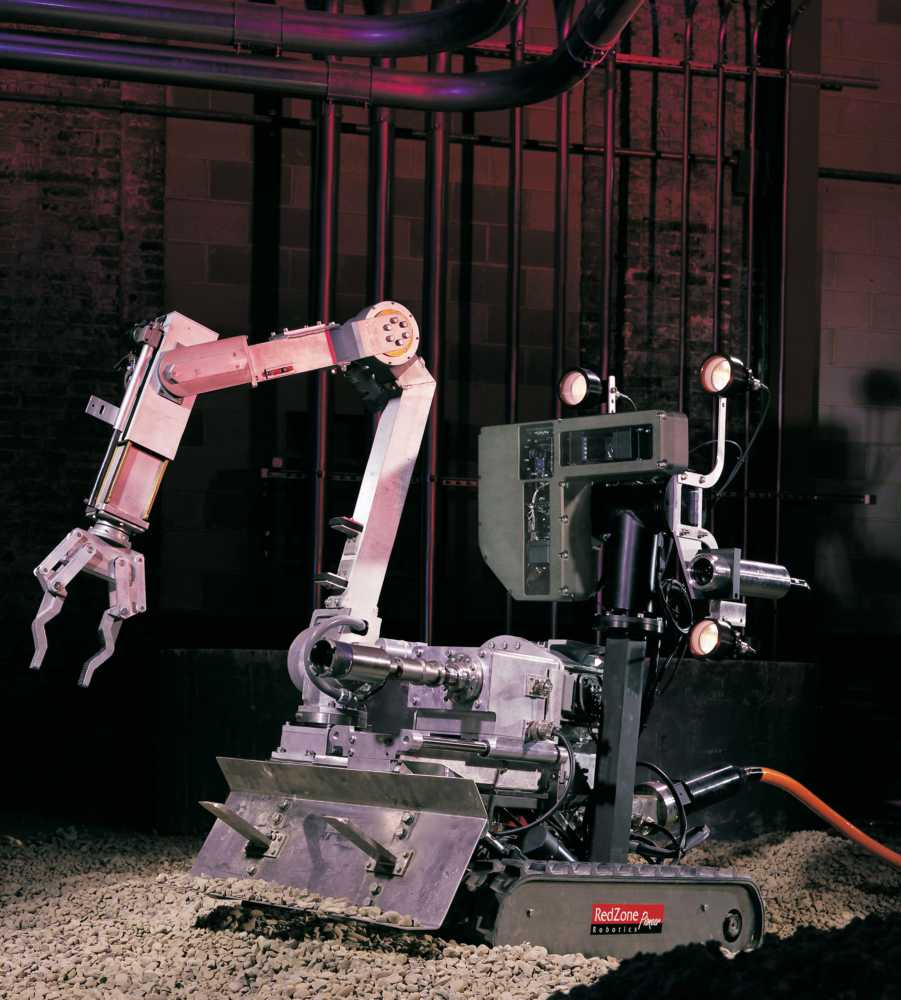
\includegraphics[width=0.8\linewidth]{images/pioneer_chernobyl}
			\caption{Pioneer robot, designed to perform hazardous teleoperated explorations in a deadly radioactive environment.}
			\label{fig:1_pioneer}
		\end{subfigure}
		\hfill
		\begin{subfigure}[b]{0.4\textwidth}
			\centering
			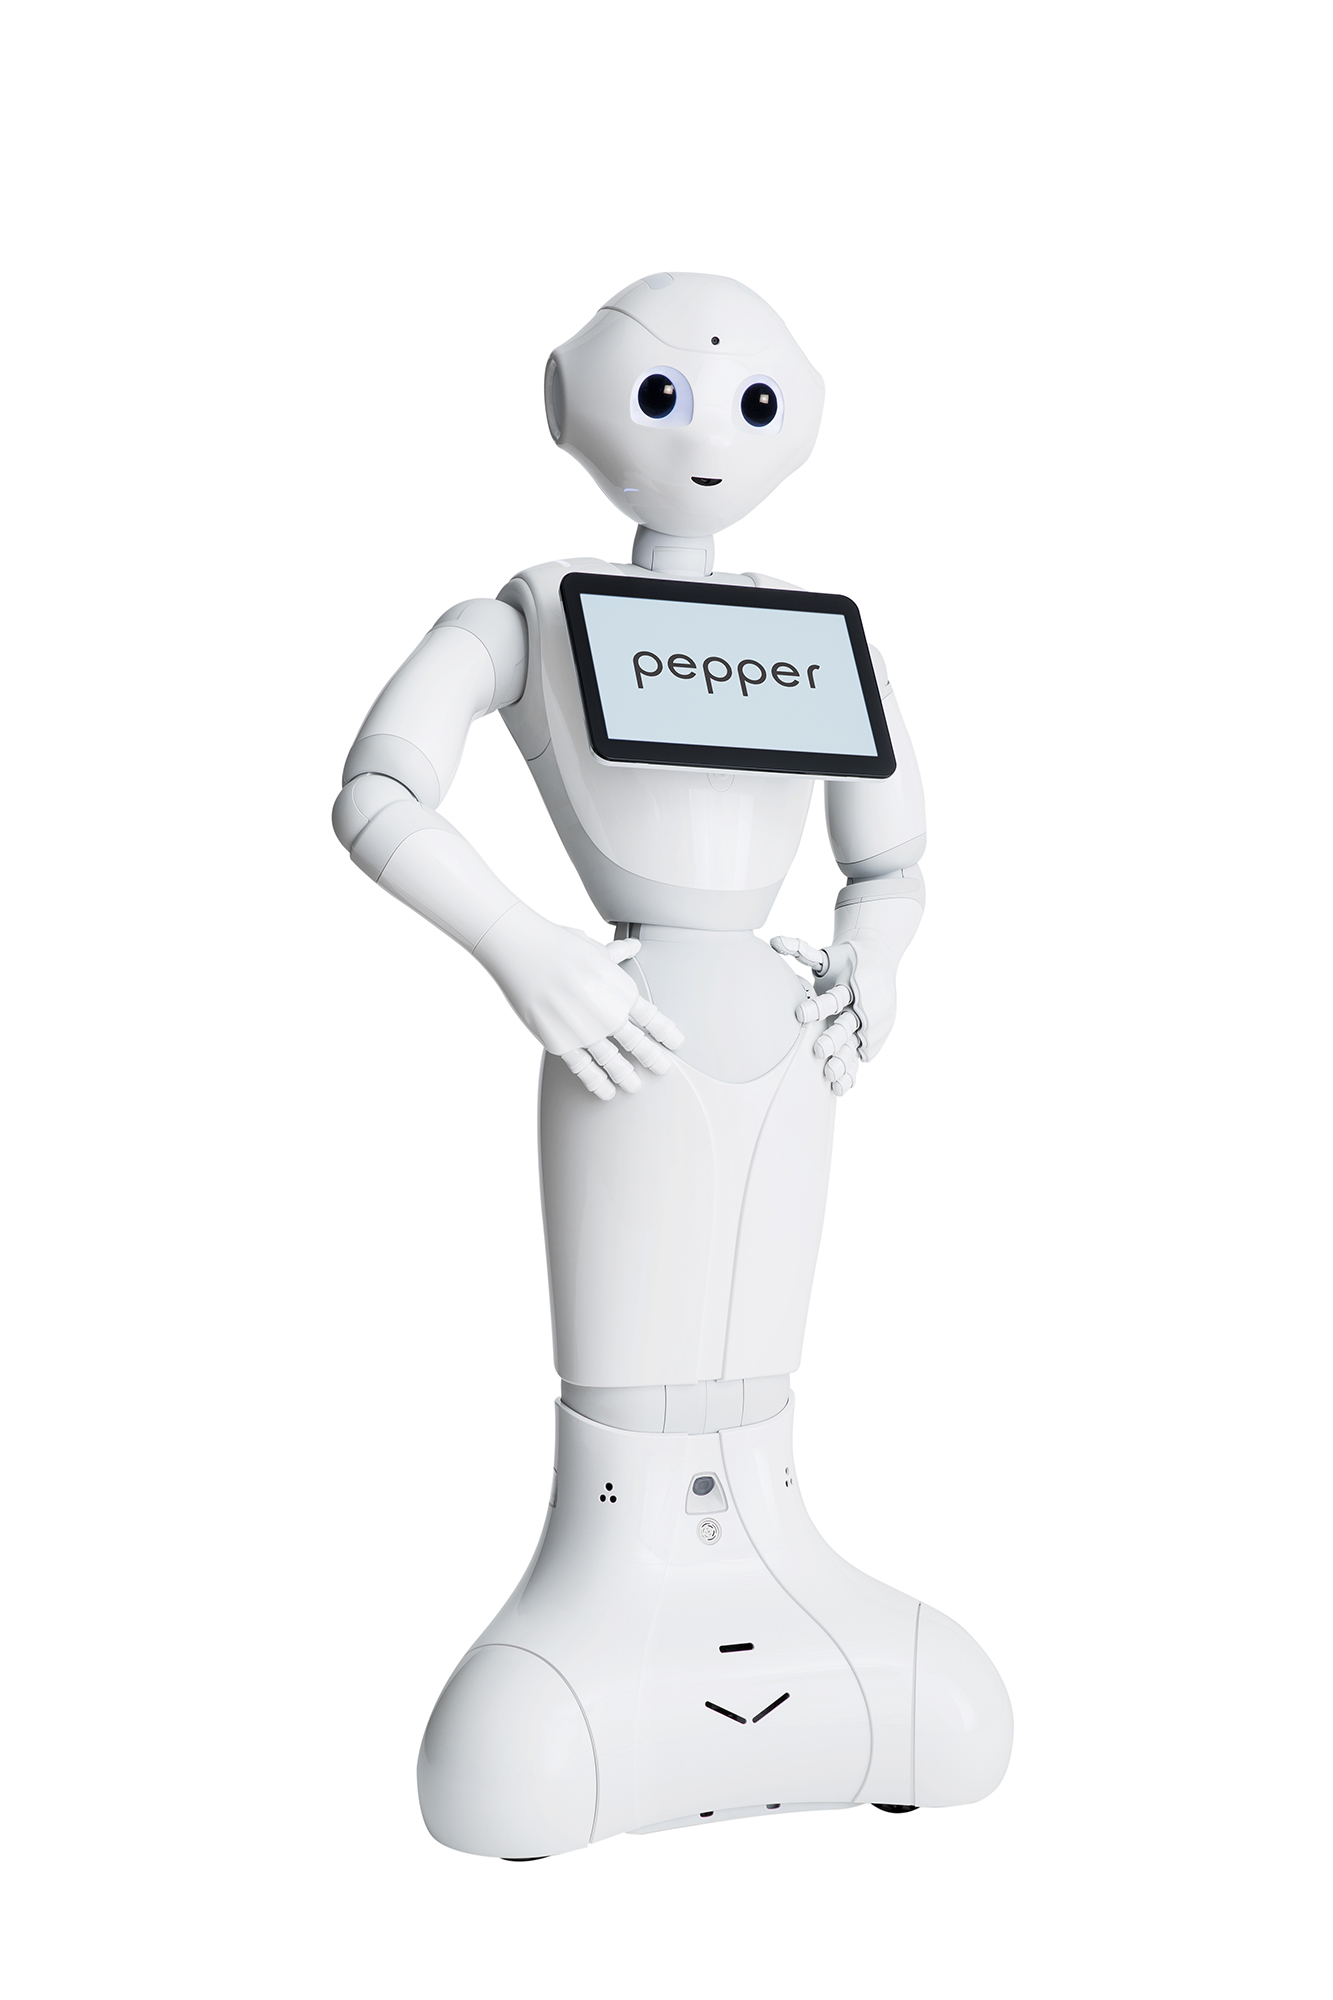
\includegraphics[width=0.8\linewidth]{images/pepper}
			\caption{Pepper, an autonomous humanoid capable of performing on board processing and reaction to external stimuli on a human way.}
			\label{fig:1_pepper}
		\end{subfigure}
		\caption{Robots of each described kind.}
		\label{fig:1_robots}
		
	\end{figure}

The important advances on the last decades on the image processing and audio recognition fields have impulsed the development of assistance systems, apart from critical machines as the previously described examples. \\

This way, several applications have arisen on people recognition and conversational behaviors, and it has been spread to everyday purposes, from personal assistants\footnote{\href{https://www.standard.co.uk/tech/google-smart-home-future-stay-a3868591.html}{Google Smart Home}}, to autonomous driving\footnote{\href{https://electrek.co/2018/06/18/what-tesla-autopilot-see-understand/}{Tesla Autopilot}}.\\


\section{Deep Learning}
\subsection{Machine Learning on Computer Vision}
Almost every time, the desired behavioral is one or more deliberated or reactive responses\footnote{A \emph{deliberated} response implies a certain level of \emph{extra intelligence}. It figures out which could be the best action to perform, considering present, past and probably future information to make the decision.\\ On the other hand, a \emph{reactive} response makes an immediate decision, depending just on what has been just perceived.}, triggered by a certain input (typically perceived by on-board sensors, among others). This raw data, which is typically retrieved on a simple way (images, audio), is processed and mapped into a concrete response. At this point, we can bring up the key question: \emph{how do we process the raw input to obtain a suitable action for the current requirements, or needings?} The answer for that question is \textit{machine learning}: the computer science field that pursues the capacity of machines to learn the suitable response to a previously unknown input. This is achieved by performing a training with a dataset of examples, which need to be properly formatted: the system has to previously know what to look for and evaluate, what is typically called \textit{features}, and learn the proper parameters for an optimum output.\\

Generally, machine learning applications on image processing can be split into two types of response (\autoref{fig:1_class_vs_det}):

\begin{itemize}
	\item \textbf{Classification:} given a set of possible classes $\{c_1, c_2, ..., c_n\}$ to which an image $x_i$ can belong, we select the class $c_i$ where $x_i$ fits the best, given a set of features extracted from it.
	\item \textbf{Detection}: given an image $x_i$, we decide if we can find or not an object/region inside of it which fits into the searched type. In the affirmative case, we locate it (using a region or a bounding box).
\end{itemize}

\begin{figure}[h!]
	\centering
	\begin{subfigure}[h!]{0.7\textwidth}
		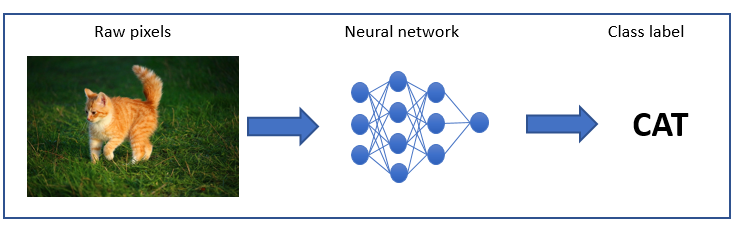
\includegraphics[width=\textwidth]{images/classification}
		\caption{Classification}
		\label{fig:1_classification}
	\end{subfigure}
	
	\qquad
	
	\begin{subfigure}[h!]{0.7\textwidth}
		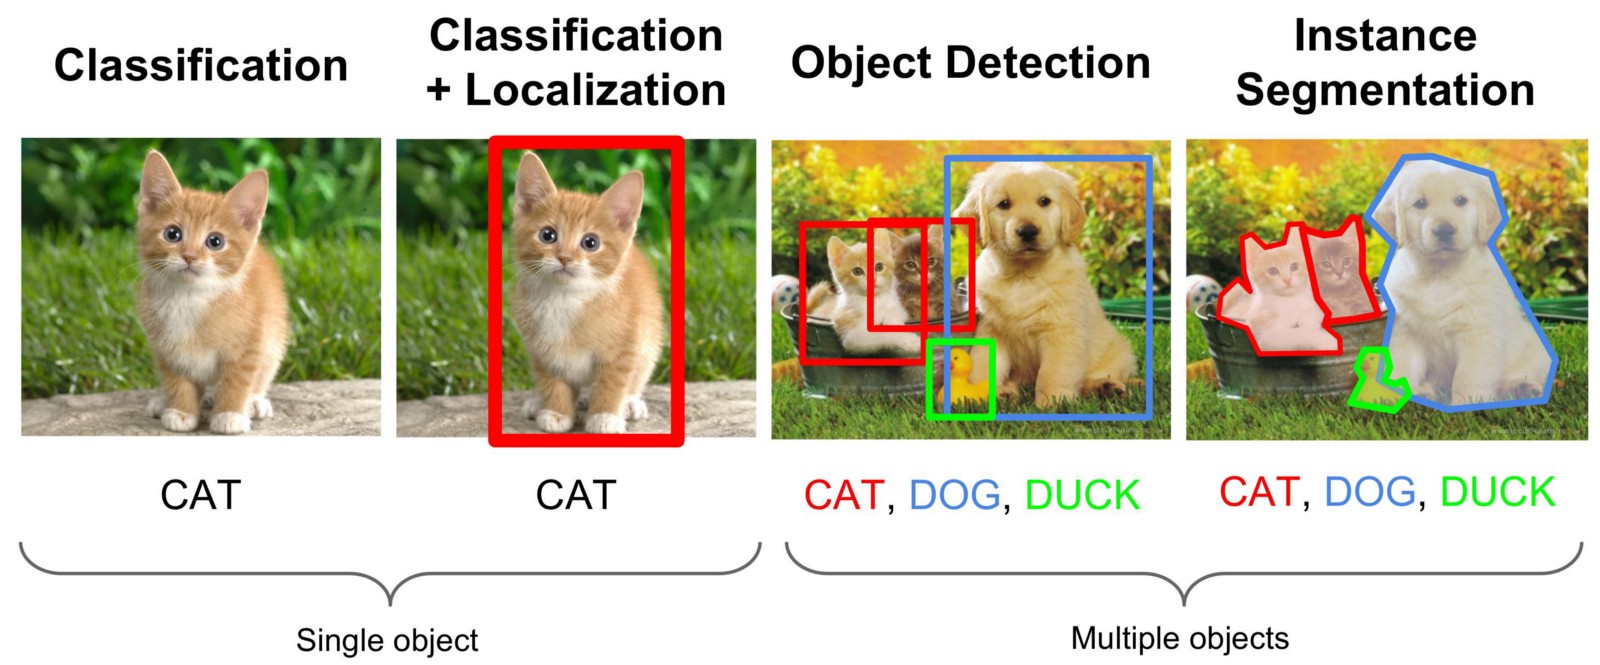
\includegraphics[width=\textwidth]{images/detection}
		\caption{Detection}
		\label{fig:1_detection}			
	\end{subfigure}
	
	\caption{Functional difference between \textit{classification} and \textit{detection}.}
	\label{fig:1_class_vs_det}
\end{figure}


\subsection{Neural Networks}
This has turned deep learning into the cornerstone of current \emph{AI} applications, which don't need complex dataset with a lot of preprocessing (that require important human effort) anymore. That simplicity is achieved through the use of \emph{Neural Networks}. A Neural Network is the representation of an algebraic algorithm which implements non-linear calculus models \cite{dl-nature}. It is composed by several processing \textit{layers}, which are made up of \emph{perceptrons}, that are generally called \textit{neurons}. This is because these neural structures \textit{emulate the human brain}, formed by a huge set of interconnected neurons, which are disposed on the already mentioned layers (\autoref{fig:1_neural_network}).\\

\begin{figure}[htpb]
	\centering
	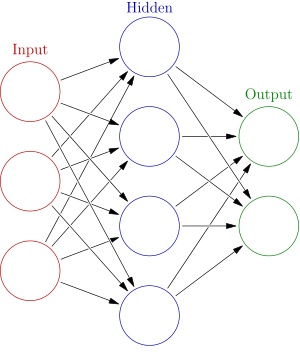
\includegraphics[width=5.5cm]{images/neural_network}
	\caption{Structure of a Neural Network}
	\label{fig:1_neural_network}
\end{figure}

First approaches to neural networks, according to \cite{nn-history} were developed on the 50s-60s decades. This was when the computational potential allowed to develop on a real machine the first modeling of the way it was believed that a brain neuron works, which was inspired by electrical circuits. These experiments \cite{first-neuron} were performed by the neurophysiologist W. McCulloch and the mathematician W. Pitts. Later, in 1949, Donald Hebb \cite{hebb} observed that the synaptic path between two neurons is reinforced (its efficiency rises up) every time it is used. This introduced the concept of \textit{training} on a neural network.

\subsection{Processing unit: the perceptron (neuron)}
\begin{figure}[h]
	\centering
	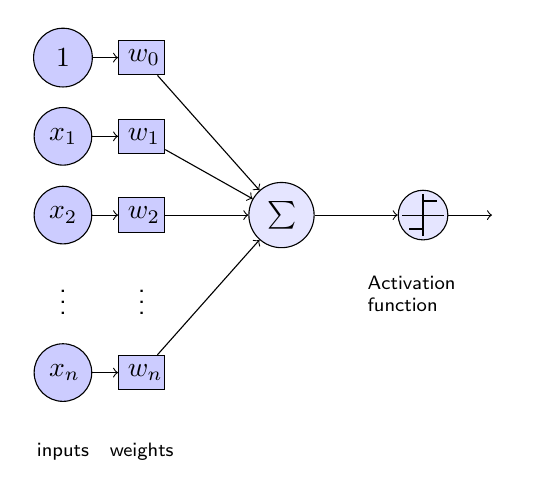
\begin{tikzpicture}
	\node[functions] (center) {};
	\node[below of=center,font=\scriptsize,text width=4em] {Activation function};
	\draw[thick] (0.5em,0.5em) -- (0,0.5em) -- (0,-0.5em) -- (-0.5em,-0.5em);
	\draw (0em,0.75em) -- (0em,-0.75em);
	\draw (0.75em,0em) -- (-0.75em,0em);
	\node[right of=center] (right) {};
	\path[draw,->] (center) -- (right);
	\node[functions,left=3em of center] (left) {$\sum$};
	\path[draw,->] (left) -- (center);
	\node[weights,left=3em of left] (2) {$w_2$} -- (2) node[input,left of=2] (l2) {$x_2$};
	\path[draw,->] (l2) -- (2);
	\path[draw,->] (2) -- (left);
	\node[below of=2] (dots) {$\vdots$} -- (dots) node[left of=dots] (ldots) {$\vdots$};
	\node[weights,below of=dots] (n) {$w_n$} -- (n) node[input,left of=n] (ln) {$x_n$};
	\path[draw,->] (ln) -- (n);
	\path[draw,->] (n) -- (left);
	\node[weights,above of=2] (1) {$w_1$} -- (1) node[input,left of=1] (l1) {$x_1$};
	\path[draw,->] (l1) -- (1);
	\path[draw,->] (1) -- (left);
	\node[weights,above of=1] (0) {$w_0$} -- (0) node[input,left of=0] (l0) {$1$};
	\path[draw,->] (l0) -- (0);
	\path[draw,->] (0) -- (left);
	\node[below of=ln,font=\scriptsize] {inputs};
	\node[below of=n,font=\scriptsize] {weights};
	\end{tikzpicture}
	\caption{Diagram of a perceptron/neuron}
	\label{fig:1_perceptron}
\end{figure}

\vspace{0.3in}
Every neuron is composed by an structured schema:
\begin{enumerate}
	\item \emph{Inputs}: the data which come into the neuron. It might come from the main stimuli, or from another neuron (as the output of the previous layer). The input for a specific neuron is called its \emph{receptive field} (which region of the total input that stimulates that particular neuron, where it looks for features).
	\item \emph{Weights}: the tuned parameters of the network. They represent the importance given to each feature on that singular neural unit. The weight $w_n$ multiplied $x_n$ times results on the contribution of the feature $n$ in the current neuron. 
	\item \emph{Sum}: the product of all the inputs with their suitable weight come into a sum operation\footnote{We consider $w_0$ as the product to the constant input $1$, as the intercept term (a constant always present independently of the current input).}, to \textit{build a total linear response:} $ z = \sum_{i=0}^{n}x_i \cdot w_i$  \footnote{There is also a summation bias term on each neuron, $b_i$, but it is ignored here for the sake of simplicity, as the weights are more representative with respect to the input.}.
	\item \emph{Activation function}: this is an crucial part of a neural network. Until now, all the numerical computations we have performed were just linear operations. If we keep the output of the neuron being a linear function of the input, we will lose the effect of having more than 1 layer, as really the total result of all the network is a linear function of the first input, so \emph{we could simplify all the network down to one single neuron}. \\
	
	For this reason, we use a \textit{non-linear activation function}, which breaks the linearity on the pipeline to provide the absolute non-linearity followed by the human brain. A typical function is the one called \emph{ReLU} (REctified Linear Unit) \cite{relu}, which follows the formula:
	\begin{equation}
		g(z) = max(0, z)
		\label{eqn:1_relu}
	\end{equation}
	
	\item \emph{Output}: when the activation function has been computed, it is forward-propagated to the output, or to the neurons belonging to the next layer. It can be seen as the importance that particular feature will have on the next neuron: if it takes nearly zero values, the next neuron will be poorly stimulated. There lies the meaning of the name of the previous component: \emph{activation function}.\\
	
	As a conclusion, we can find that the general output of a neuron $a(z)$ as:
	\begin{equation}
		a(z) = g(\sum_{i=0}^{n}x_i \cdot w_i)
	\end{equation}
	
	This will be the new data (\emph{receptive field}) that will be introduced on a neuron or set of them from the next layer.
\end{enumerate}

\subsection{Deep Neural Networks}

\emph{Deep learning} is the piece of machine learning that is capable to \textit{automatically learn the features that the system could use from primary data} (pixels on images, samples on audio, words in text processing, etc.).\\

The fact of having more than one layer gives to the network the concept of \emph{depth}. This opens the door to a vast set of possibilities, as \textit{it allows us to perform deep learning with neural networks: Deep Neural Networks}. This can be achieved, as we can see on \autoref{fig:1_deep_nn}, by introducing a new kind of layer, where all the new neurons are connected to every single neuron of the previous one.\\
This is typically called a \textit{fully connected layer}, and the fact of relating every single activation from the previous layer with a set of tunable weights on each neuron allows to rapidly find common patterns followed by features seen on one of the analyzed scenarios (e.g. syntactical relationships between several kinds of words in language processing, or finding edges or shapes on image detection/classification).

\begin{figure}[h]
	\centering
	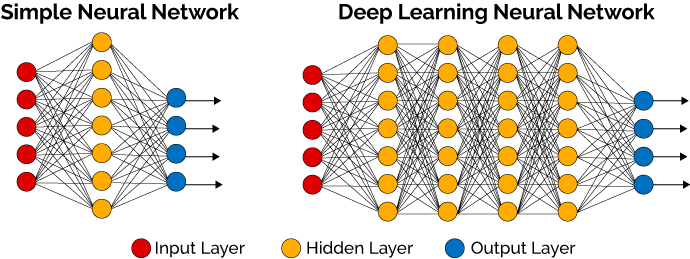
\includegraphics[width=0.9\linewidth]{images/deep_neural_network}
	\caption{Evolution to a \textit{deep} neural network.}
	\label{fig:1_deep_nn}
\end{figure}

\subsection{Convolutional Neural Networks (\emph{CNNs})}
\label{sec:1_cnn}

Finally, this leads us to the last concept we will study on this dissertation. As we have said before, we can connect a big set of neurons between themselves to extract more abstract and complex features, of increasing interest with the number of neurons and layers.\\
 
If we aim to apply this processing to images (\textit{Computer Vision}), we have to take into account that, if we want to input an image into a neural network, each pixel has to be taken as an input, and also the fact that an RGB image is composed of 3 channels (1 channel per color), so, for an image with a dimensions of $m$ pixels wide and $n$ pixels high, we will need $m\cdot n \cdot 3$ input neurons. Besides this considerable number, we will have to take into account the neurons resulting on the additional deeper layers that we will add to have an high enough abstraction level for our application. This drives to absurd numbers of simultaneous neurons working, that are difficultly handable during a feed-forward execution, but absolutely unfeasible on a training process. An additional problem can be a moving object/region on the image: we must be capable to detect the shape of a car on the right side of the image, or in the left one.\\

We can solve both problems simultaneously with an easy procedure: we will not process the entire image at one time. Instead of that \textit{we will perform a convolution operation (\autoref{fig:1_convolution}) between the inputs of our network, and different regions of the image}, sliding and multiplying a \emph{parameterized mask} along the whole image. This operation is performed with the objective of the product returning a high value on the interesting regions of the image. This will output \emph{activation maps}, which symbolize the response of that portion of the image to the weight mask. This can be performed, as we have said before, a few times with different masks to obtain features with a higher degree of abstraction. As we want to keep the computational complexity low, we can alternate these layers with \textit{pooling layers}, which subsample the resulting maps, to keep it simple (if we keep only 1 of each 3 pixels of an activation map, selecting it carefully to retain the maximum information, we can reduce the number of necessary neurons on the next layer on a factor of $\frac{1}{3} \cdot \frac{1}{3} = \frac{1}{9}$). This is reflected on \autoref{fig:1_cnn}, where the process of convolution-pooling can be repeated a few times, and then the result (which should not have considerably big dimensions) are inputted into a fully connected layers, to extract and handle the relations between the features and the possible classes (on a classification scenario).\\


\begin{figure}[h]
	\centering
	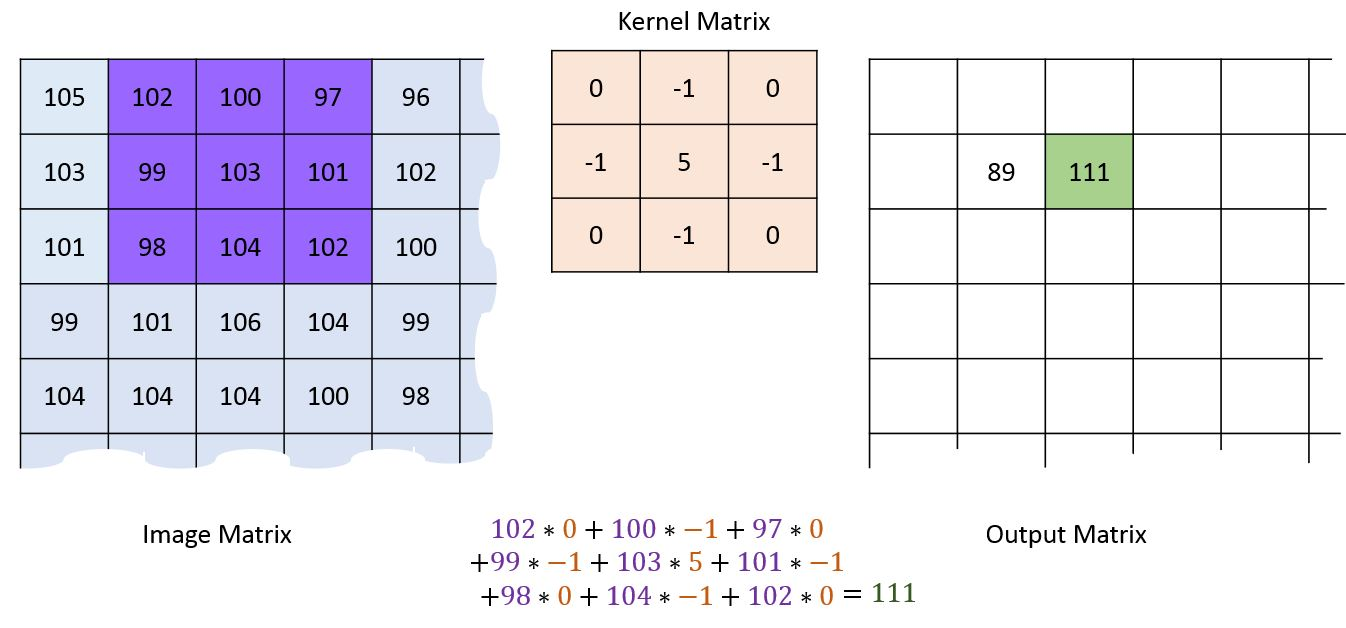
\includegraphics[width=5in]{images/convolution}
	\caption{Convolution operation applied on an image (image from \cite{image-convolution}).}
	\label{fig:1_convolution}
\end{figure}





But, \emph{how do we find the best value for each weight, and for each layer?} That's the process we call \textit{training a network}. Using a technique called \emph{back propagation}, we can compute the most suitable values for every neuron in the network.\\

\begin{figure}[h]
	\centering
	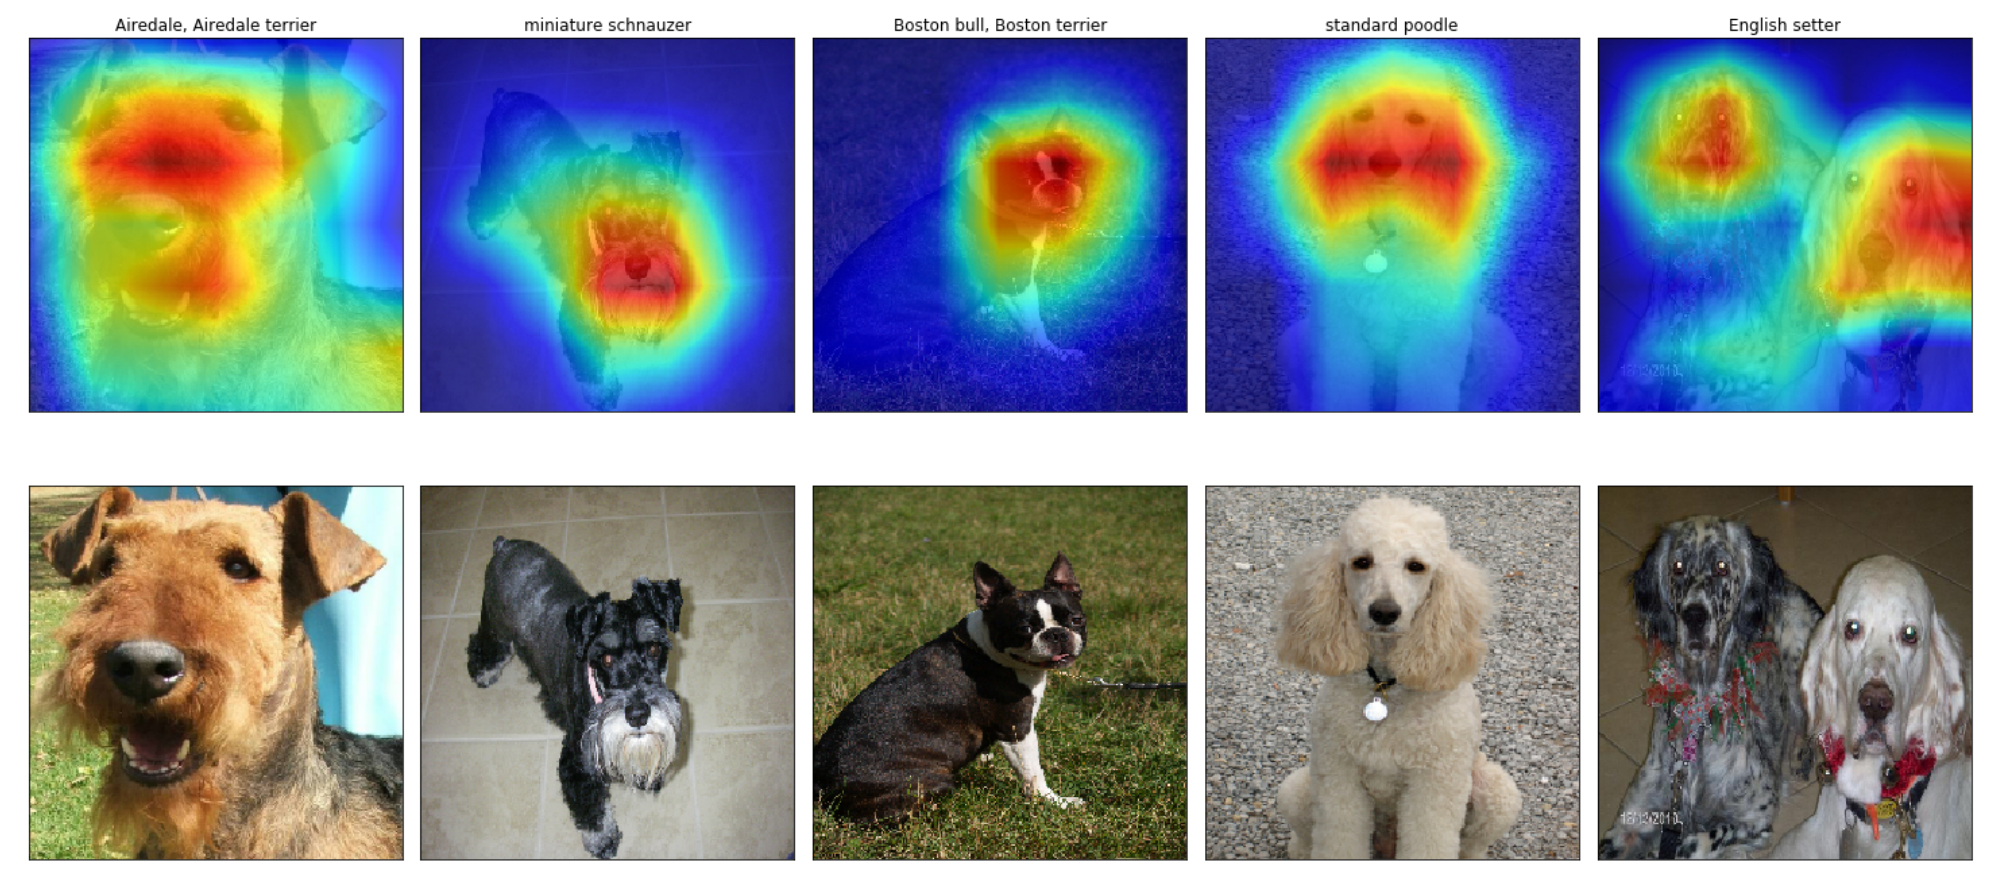
\includegraphics[width=0.9\linewidth]{images/activation_maps}
	\caption{Activation maps of a detection CNN searching for dogs on different images \cite{activation-maps}.}
	\label{fig:1_activation_maps}
\end{figure}



\begin{figure}[h]
	\centering
	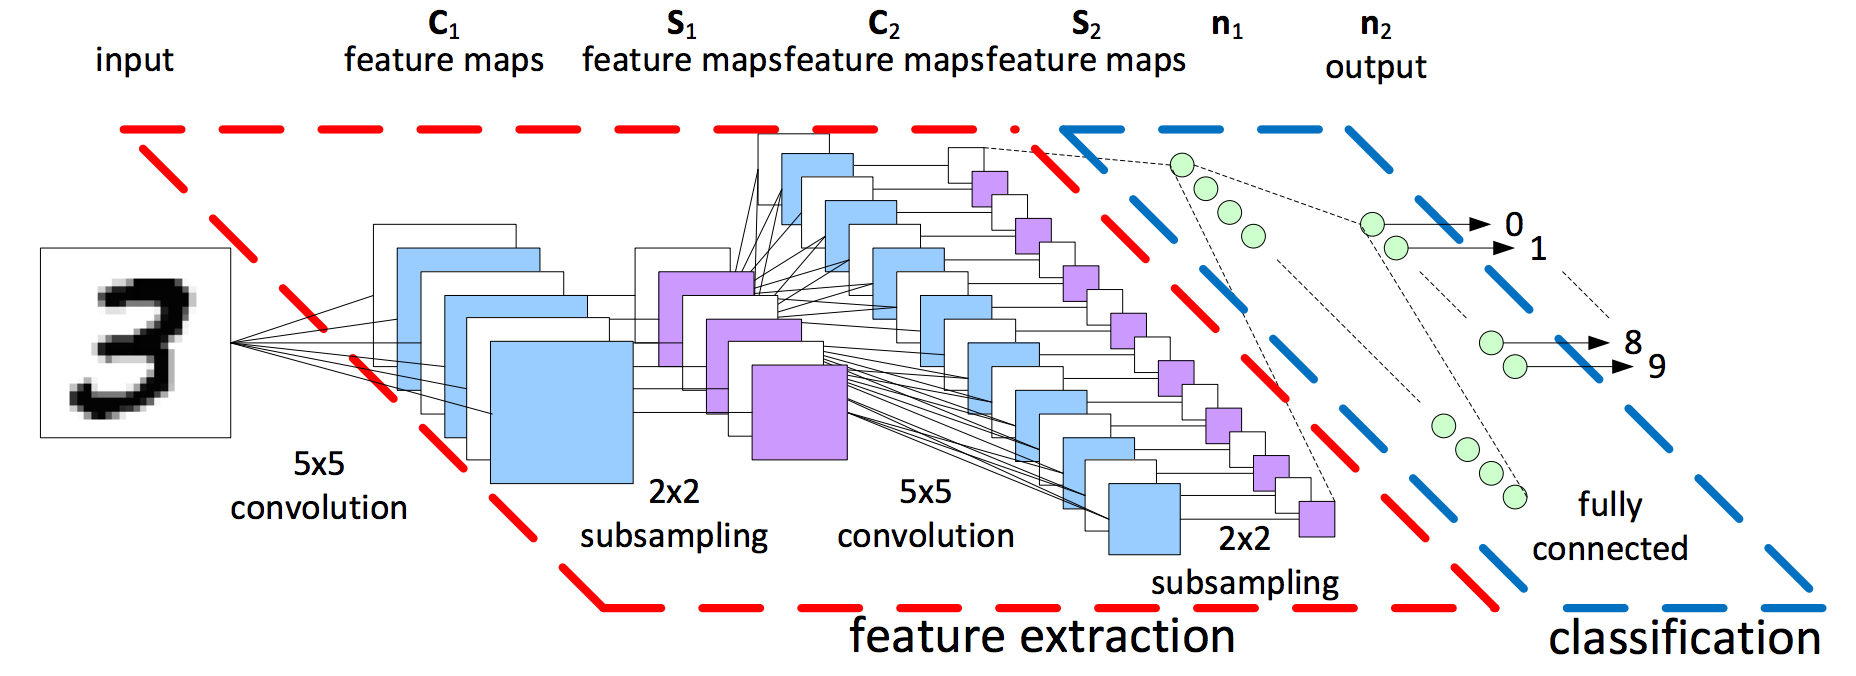
\includegraphics[width=0.9\linewidth]{images/cnn}
	\caption{Schematic of a CNN.}
	\label{fig:1_cnn}
\end{figure}

\section{Deep Learning on JdeRobot}
\label{sec:dl_jderobot}
So, as we have been describing, Deep Learning can be of a great interest on the image processing field, as it allows to implement an easy and really robust AI algorithm.\\

JdeRobot\footnote{\url{https://jderobot.org}} is an open-source software development suite, built from  this University, and among all the developed software/investigation inside it, we can find some interesting programs/projects for our purposes:

\begin{itemize}
	\item \texttt{Detection Suite}\footnote{\url{https://github.com/JdeRobot/dl-DetectionSuite}}: it is a C++ application, suitable to load/benchmark \textit{detection} Darknet/YOLO\footnote{\url{https://pjreddie.com/darknet/}} models, against different databases. It is also capable, through a Python$\rightarrow$C++ interface, to load TensorFlow/Keras models as well.
	
	\begin{figure}[h]
		\centering
		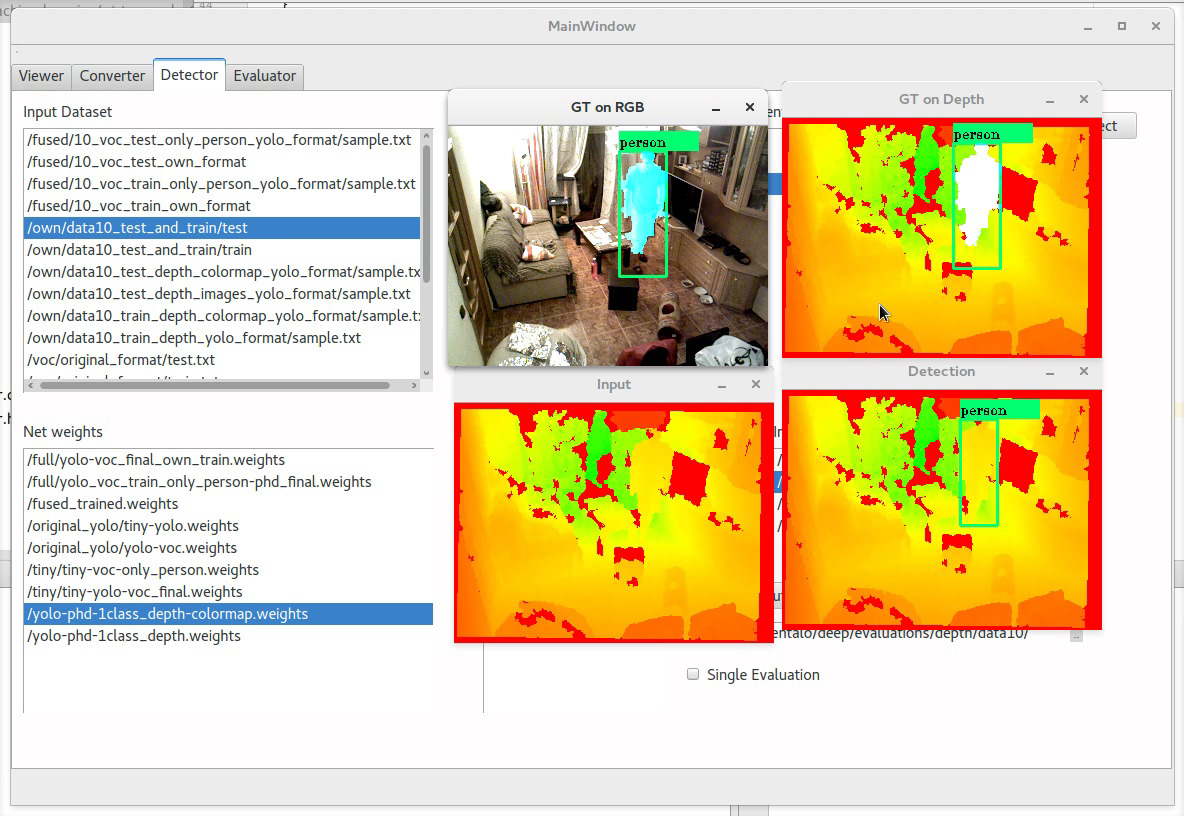
\includegraphics[width=4.5in]{images/detection_suite_depth}
		\caption{\texttt{DetectionSuite} on action.}
		\label{fig:1_detectionsuite}
	\end{figure}

	\item Final project of David Pascual \cite{dpascualhe} and Nuria Oyaga \cite{noyaga}: a further study of Deep Learning, applied on Python (Keras and Caffe frameworks, respectively) to \textit{digit classification} (\autoref{fig:1_digitclassifier}) implementing a CNN as it has been seen.
	
	\begin{figure}[h]
		\centering
		\begin{subfigure}[h]{0.45\linewidth}
			\centering
			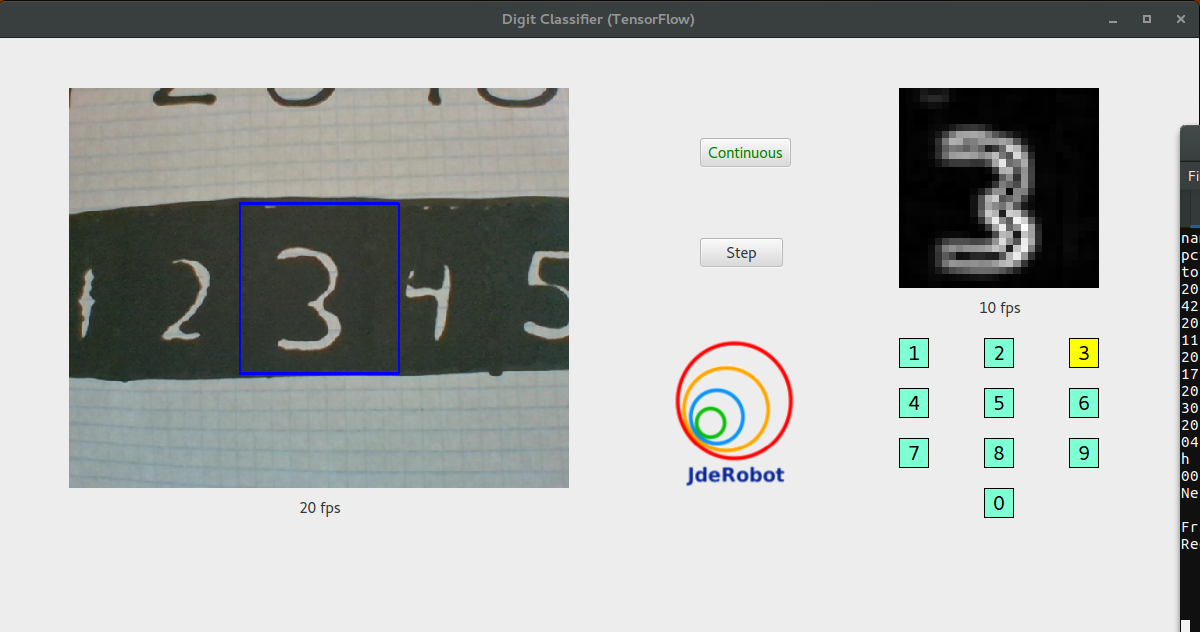
\includegraphics[width=2.7in]{images/digitclassifier}
			\caption{\texttt{DigitClassifier} working.}
			\label{fig:1_digitclassifier}
		\end{subfigure}
		\qquad
		\begin{subfigure}[h]{0.45\linewidth}
			\centering
			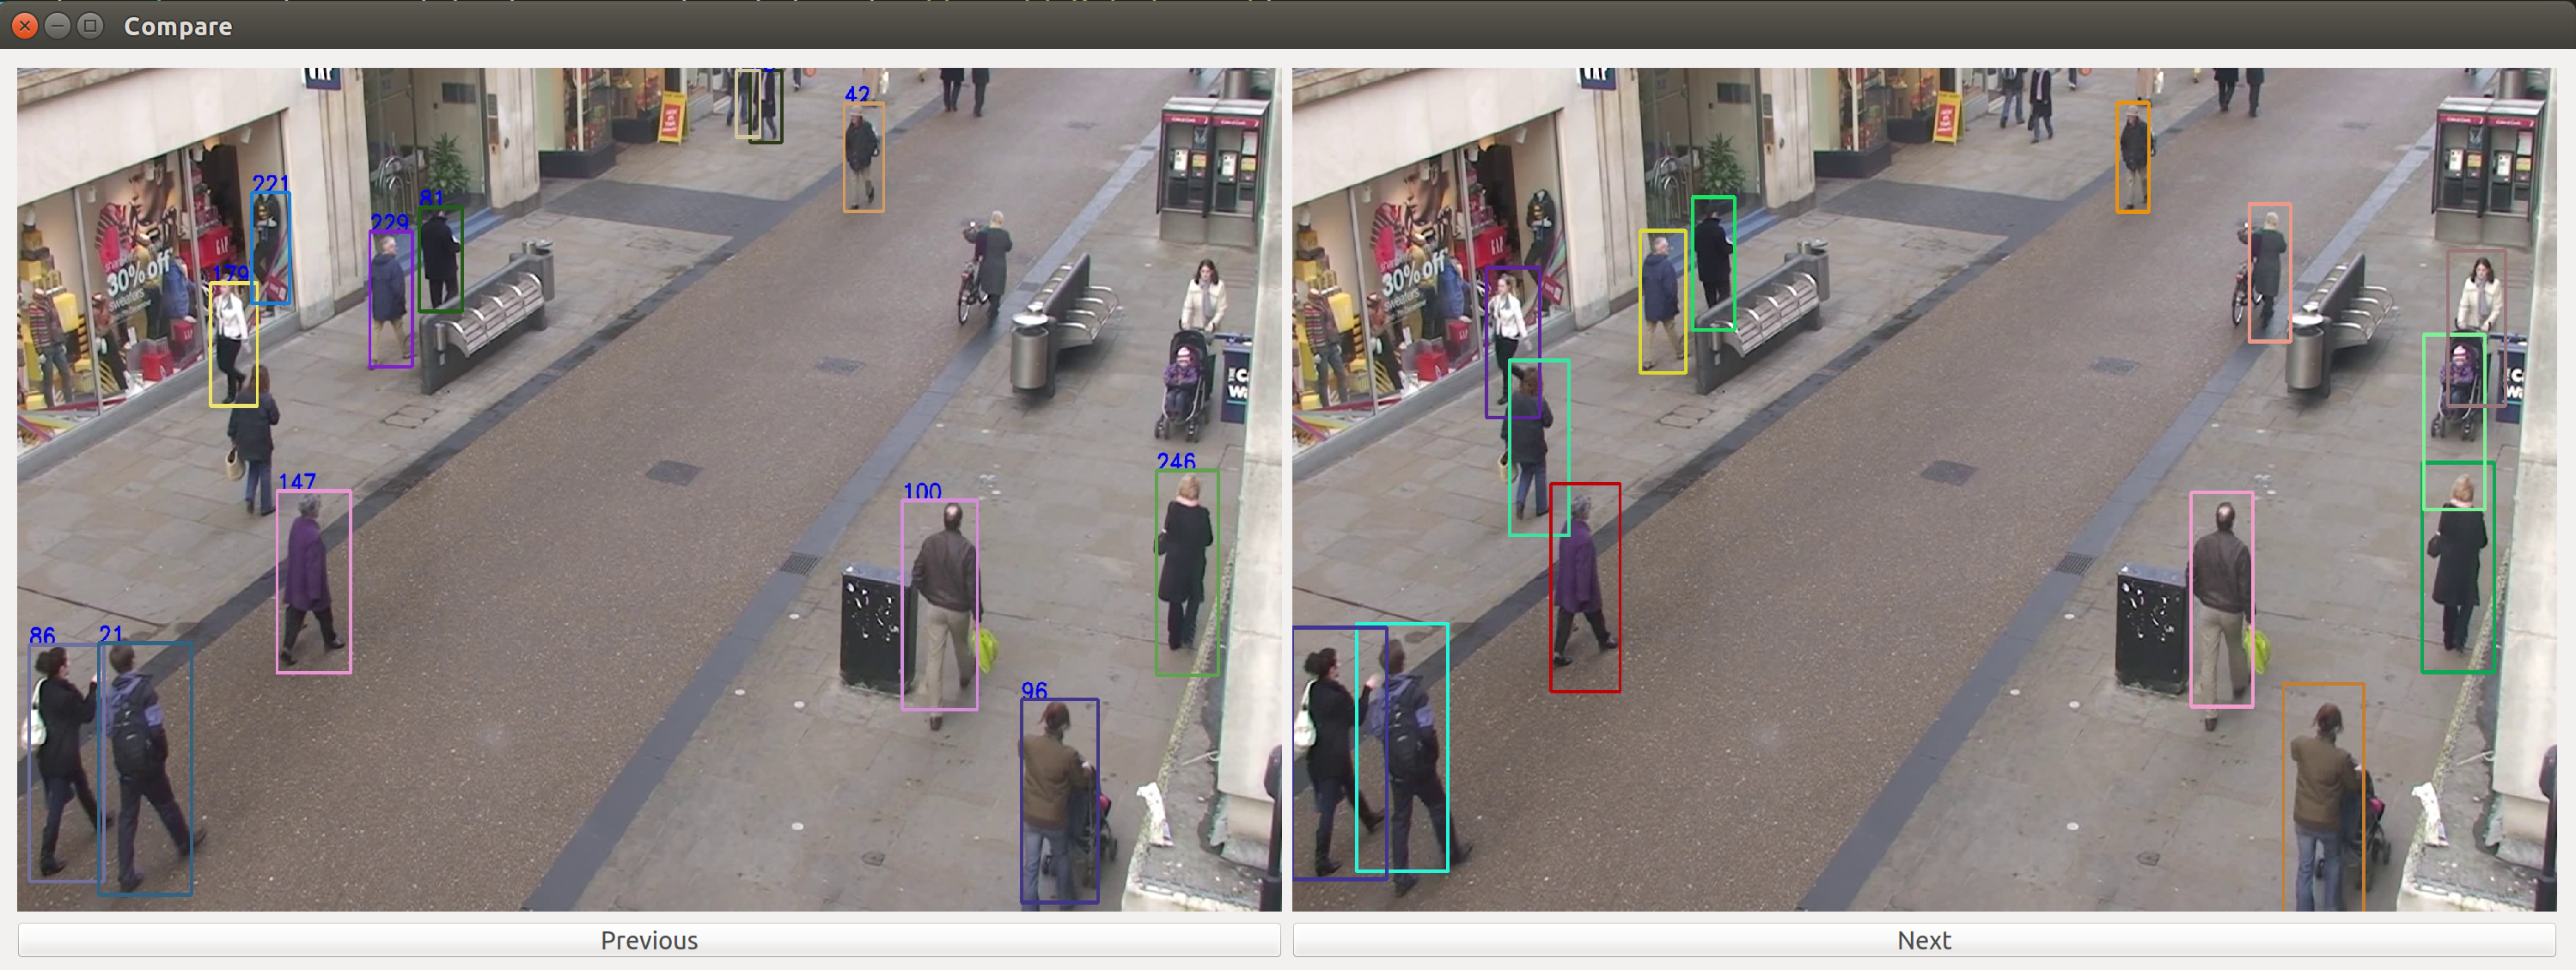
\includegraphics[width=3.7in]{images/marcos_people_tracker}
			\caption{\texttt{PeopleTracker} working.}
			\label{fig:1_people_tracker}
		\end{subfigure}
		\caption{Some JdeRobot student projects on action.}
		\label{fig:1_jderobot_projects}
	\end{figure}

	\item MsC project of Marcos Pieras \cite{marcospieras}: On this master thesis, an application implementing two neural networks (as we will do) has been developed. One of them allows us to \textit{detect} people on an image, and the other one (a siamese network, as we will describe later) can track features of each person, to keep every detected individual identified on a surveillance image system (and possibly trace the route followed by each person) (\autoref{fig:1_people_tracker}).
\end{itemize}

In conclusion, as we have been mentioning and been taking a glance on the possible applications, Deep Learning can make such a brilliant tandem along with a reactive behavioral. We have taken a glance on a few possible applications, and the following dissertation will struggle to demonstrate it.\\




\begin{center}
	\textbf{Robotics + deep learning rock!}
\end{center}



	
	
	%%%%%% OBJECTIVES %%%%%%
	\chapter{Objectives}
Once we have presented the introductory context of this project, we will describe its objectives, along to the followed methodology to achieve all of them.\\

The final objective is to enrich the JdeRobot platform on its Computer Vision aspect, upgrading an existing component and creating two consecutive new ones. Keeping this in mind, we will be able to generate a behavioral focused, as a specific application, on tracking and actively following a person, making use of a robot. This internal process of transformation of the stimuli into a reactive movement will be accomplished using \textit{Convolutional Neural Networks}.\\


\section{Main objectives}

		\subsection{Classification}
			Our first objective (and the first task to tackle) will be to upgrade the support of the digit classification tool already present in JdeRobot, \texttt{DigitClassifier} (\autoref{sec:3_digitclassifier_jderobot}). This will allow us to make the scope of this component bigger, due to the support for the new framework, TensorFlow (\autoref{sec:3_tensorflow}). This is a good starting point to achieve some initial skills building and training Convolutional Neural Networks on TensorFlow (it will be the main framework used all along the project).\\
		
		
		\subsection{Detection}
			As it will be described on the suitable chapter, we will build a component (\texttt{ObjectDetector}) which deploys \textit{a generic object detection algorithm} on an incoming video stream. This component will be ready to work in \emph{real time}. It will also be compatible with new network models (e.g. a new detection model trained by us), which will be loaded transparently at runtime.\\
			
			As it can be inferred, it will not provide a response \textit{per se}. Its visible output will be to draw \emph{bounding boxes} surrounding each detected object, indicating as well the class where that particular object belongs (person, airplane, dog, etc.), and its score (confidence in \%).\\
		
		\subsection{Tracking and following}
			As an example of the plethora of possible applications of the previous described objective/milestone (object detection on an image), we want to implement a ``person following" behavioral. Our main objective here is to \textit{identify and track} the person to follow, which will semantically be called \emph{mom}. The component that comprehends the previous detection behavioral and this new one will be named \texttt{FollowPerson}. The great advantage here is the strength a CNN can achieve under variable light conditions. That makes this technique perfectly suitable to command physical actuators on a robot.\\
			
			We will make use of the detected people (with the technique followed on the previously described node and constraining the result to only retain people detection), and look for the face of each one of them. Later, we will make use of another neural network technique, called a \emph{siamese network} (it will be properly explained later) to identify them. It will allow us to find \emph{mom}, in case it is being seen by the camera, and command a proper response to the robot with the objective of following \emph{mom}.\\
			
			\vspace{1in}

As we have said before, these two last nodes/components are successive. Thus, they will share an important part of the global objectives.\\

We will start breaking down the common objectives between both applications, into three functional blocks:

\begin{itemize}
	\item \textit{Design:} both milestones have been preceded by a first \textit{documentation} phase. While the theoretical base was learned and achieved, some papers and examples were investigated. We will go some deeper in each section.
	
	Later, a more specific design phase will be to specify the structure of the nodes.
	From now on, we will have to perform several tasks simultaneously:
	\begin{itemize}
		\item Grabbing the incoming image(s) from the sensor(s).
		\item Processing the image(s).
		\item Properly update the GUI (\textit{Graphical User Interface}) with the image(s) and the outputs of the processing.
		\item \textit{Only on the following node:} send the computed response order to the actuators.
	\end{itemize}
	%
	These tasks should follow an \emph{asynchronous schema} every time, to avoid blocks between tasks, and taking advantage of some shared memory to exchange inputs/outputs. Besides, this allows us to have a custom iteration period for each task: we shouldn't have to wait until the neural network finishes feed-forwarding the image to refresh the \emph{GUI}. On a high level structure, it could follow the schema on the \autoref{fig:2_tasks}.
	
	\begin{figure}[h]
		\centering
		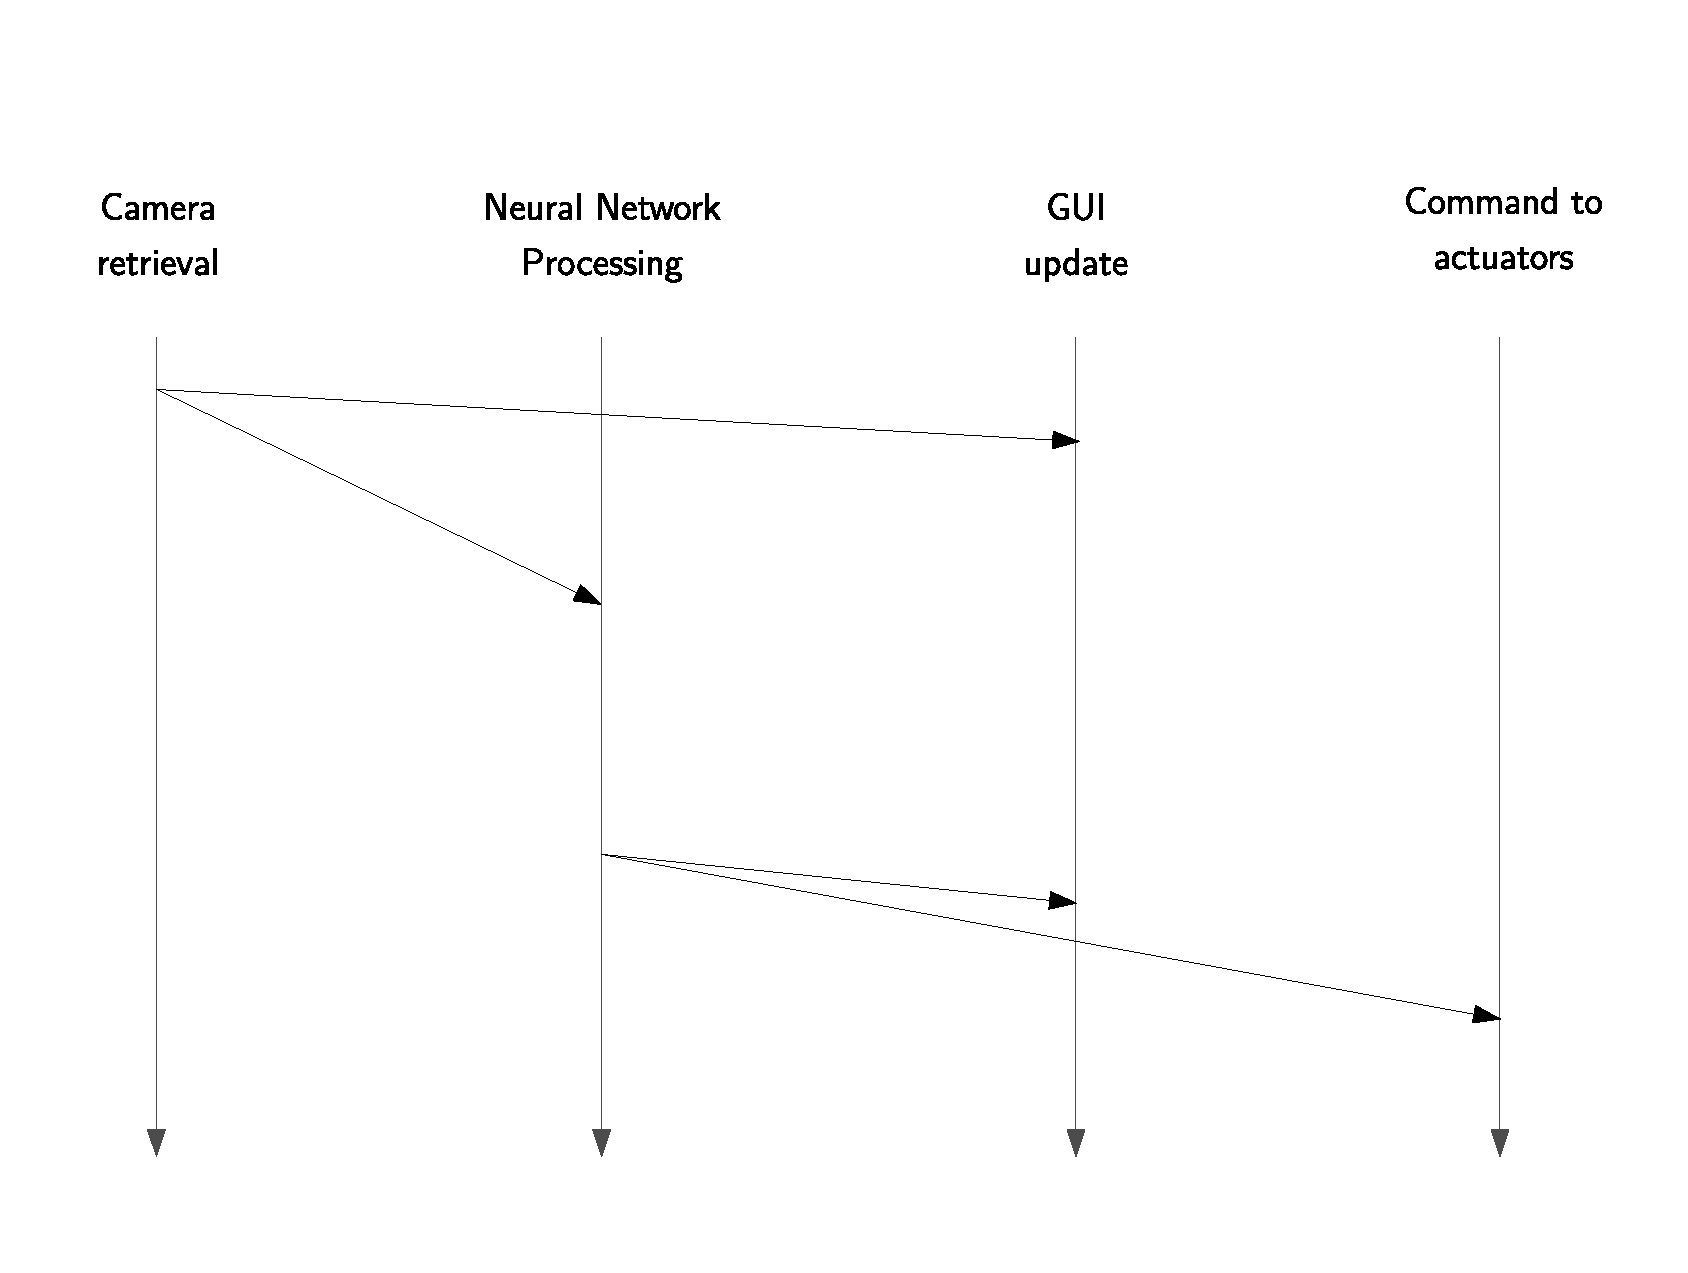
\includegraphics[width=4in]{images/tasks_threads}
		\caption{Parallel tasks to perform, and data exchange between them.}
		\label{fig:2_tasks}
	\end{figure}
	
	\item \textit{Implementation:} the next and most time consuming objective is to \textit{develop both components}. The advantage is, once again, that both components are successive. This makes code reutilization a very interesting move, as we will only need to perform a language-friendly additions (on a simple way, thanks to \textit{Object Oriented Programming})) to the \texttt{Object Detector} code to implement the \texttt{Follow Person} features (depth images support, computing and commanding movements to the motors, among others). Details will be described on the appropriate section.
	
	\item \textit{Experimentation\footnote{\textit{"In theory, theory and practice are the same. In practice, they are not."}, Y. Berra}:} these nodes have a very strong tunability component (from neural network parameters to movement factors in the commands for the motors, stopping over describing all the desired behavior that the following algorithm has to adopt in several situations that it has to be capable of handling).
	
\end{itemize}

Finally, we will briefly highlight the \textit{personal} objectives we have pursued on this project. As this has been developed along a whole year, and on a relatively abstract field as \emph{deep learning} is, a level of rigour has been necessary to accomplish satisfactory results. This provides a novice investigator the opportunity to learn about the phases and development process on a much more professional way than a homework task. \\

In addition, this project has allowed an interested person in \emph{deep learning} to learn about a cornucopia of concepts and experience. Later, when it was decided to evolve towards creating a reactive behavioral, it was motivating to make the most of a possible synergy between two different fields of knowledge, as \emph{deep learning} and \emph{robotics} are. It has to be remarked that the implementation of the development has always been possible, so it has been easy where there was more work to do in every moment.

\section{Methodology}
The development of this project, as it has been described, has been subdivided into smaller tasks, or \emph{prototypes}, which could be addressed as individual tasks to achieve. The way to tackle them has been a \textit{spiral methodology} \cite{boehm-spiral}.\\

\begin{figure}[h]
	\centering
	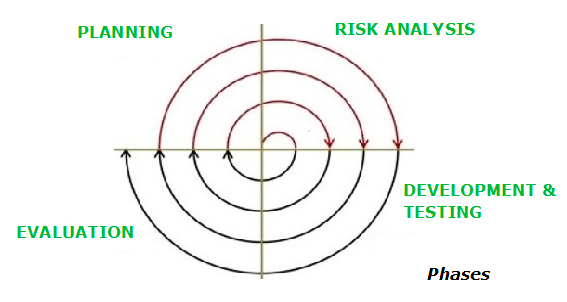
\includegraphics[width=4in]{images/spiral}
	\caption{Spiral Development Model.}
	\label{fig:2_spiral}
\end{figure}

This consists on a software development work procedure that, on a general outline, is very similar to a conch. It describes a 4 phases methodology \cite{spiral-steps}, explained right below:

\begin{enumerate}
	\item \textit{Planning:} establishing the objectives to tackle on the incoming work iteration.

	\item \textit{Risk Analysis:} Later, we evaluate the possible risks and dangers we can find developing the specific program(s). For each found risk, we will try to find a solution to solve or, at least, mitigate it beforehand.

	\item \textit{Development \& testing:} This phase is purely focused on writing the planned piece of software, following the guidelines obtained on the previous steps. In addition, corresponding tests should be performed to check that the work will accomplish the asked functionality.
	\item \textit{Evaluation:} Lastly, when the development phase has been finished, an evaluation has to be performed on the results. This will be the key to know if it is compliant with the initial requirements and if, hence, its development has been successful.
\end{enumerate}

As this was the general procedure followed for each iteration of the developed software, the completion of the evaluation phase immediately led to another planning phase, already belonging to the next iteration. As this is a cyclic process, we can perform as many iterations as desired, slightly increasing the scope of the project on each new one.\\

The workflow present on this project has been supported by weekly meetings, scheduled in order to get up-to-date with the last established objectives and tasks, and set up the work until the next one. This has allowed to keep a constant feedback with the tutor and hold the followed path onto the desired direction.\\

Additionally, a MediaWiki page\footnote{\url{https://jderobot.org/Naxvm-tfg}} has been mantained on the JdeRobot website, reflecting every effort and achievement in order to have a good temporal reference of the work done, and a timeline of accomplishments, and including demonstration videos for each successful iteration result.\\

The code for all the project has been handled on the GitHub repository\footnote{\url{https://github.com/RoboticsURJC-Students/2017-tfg-nacho\_condes}} created for this purpose. However, as the resulting nodes were officially incorporated to the JdeRobot environment, they were migrated to their own repositories. This will be further described on the section dedicated to each component/iteration.\\

	
	%%%%% INFRASTRUCTURE %%%%%
	\chapter{Infrastructure}

\section{Hardware}
	\subsection{Sony EVI D100P}
		\begin{figure}[h]
			\centering
			\begin{subfigure}[h]{0.4\linewidth}
				\centering
				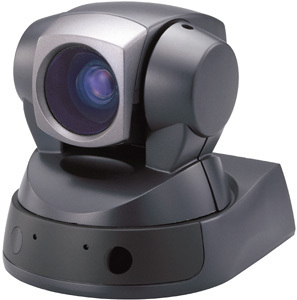
\includegraphics[width=1.6in]{images/ptz_front}
				\caption{Front side.}
			\end{subfigure}
			\qquad
			\begin{subfigure}[h]{0.4\linewidth}
				\centering
				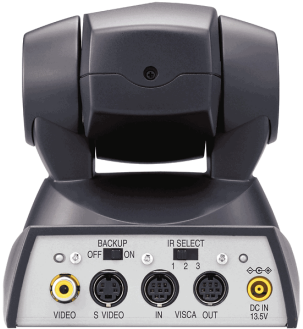
\includegraphics[width=1.6in]{images/ptz_back}
				\caption{Back side.}
			\end{subfigure}
			\caption{Sony EVI D100P.}
			\label{fig:3_evi}
		\end{figure} 
		
		The first hardware element that we used is the Sony EVI D100P\footnote{\url{https://pro.sony/en_IN/products/ptz-network-cameras/evi-d100-d100p-pal-}}. It is a \emph{PTZ} cam (which stands for \emph{Pan Tilt Zoom}). It is a camera which, originally thought and designed for videoconferences, is equipped with a bunch of precision motors. This allows it to be teleoperated, performing a soft and steady two-dimensional movement on demand:
		\begin{itemize}
			\item \emph{Pan:} horizontal movement. It can take values from $-164º$ to $164º$ from the centered position. This movement can be performed at a certain speed, which can be setted between $1$ and $24$.

			\item \emph{Tilt:} vertical movement. Its range goes from $-30º$ to $30º$, and the movement speed can be also varied between $1$ and $20$.
		\end{itemize}

		The low-level implementation of the movement commands is the \emph{VISCA} protocol, a propietary solution from the manufacturer (Sony). It is received by the cam through a RS-232C (the traditional low-rate serial interface before USB extended), so we can connect it to a modern computer with a RS232-USB interface.

		However, the driver that controls this camera (\ref{sec:3_evicam_driver}) does not offer support for a \emph{zoom} movement, but it is not very relevant for this application.\\

		As the video sensor is an analogue device, we need to convert it to a digital format. We achieve this with a video capture device, which outputs video in a digital format. This image flow will be processed by a ROS driver (\autoref{sec:3_usb_cam}), that will be later explained.\\

		Something remarkable about this device is that it is a bidirectional device: we \textit{receive} images from its camera, and, at the same time, we \textit{send} it commands to move the motors.\\
		
		As we can infer from the described technical specifications, this is a relatively old device, so we have to be careful on the movement commands. This is due to the short period of position update: even if we command the motion action at the maximum available speed, the movement won't complete before the next update is commanded. In addition, the camera mantains a buffer of the pending commands to be updated. Hence, sending absolute movement commands (\autoref{fig:3_ptz_wrong}) will result in a chaotic behavior of the camera.\\
		
		So, we have needed an alternative approach, consisting of \emph{differential} movements (\autoref{fig:3_ptz_right}). This has the objective of ensuring its completion before the next iteration comes in, so we will perform it at the maximum available speed.

		\begin{figure}[h]
			\centering
			\begin{subfigure}[h]{0.4\linewidth}
				\centering
				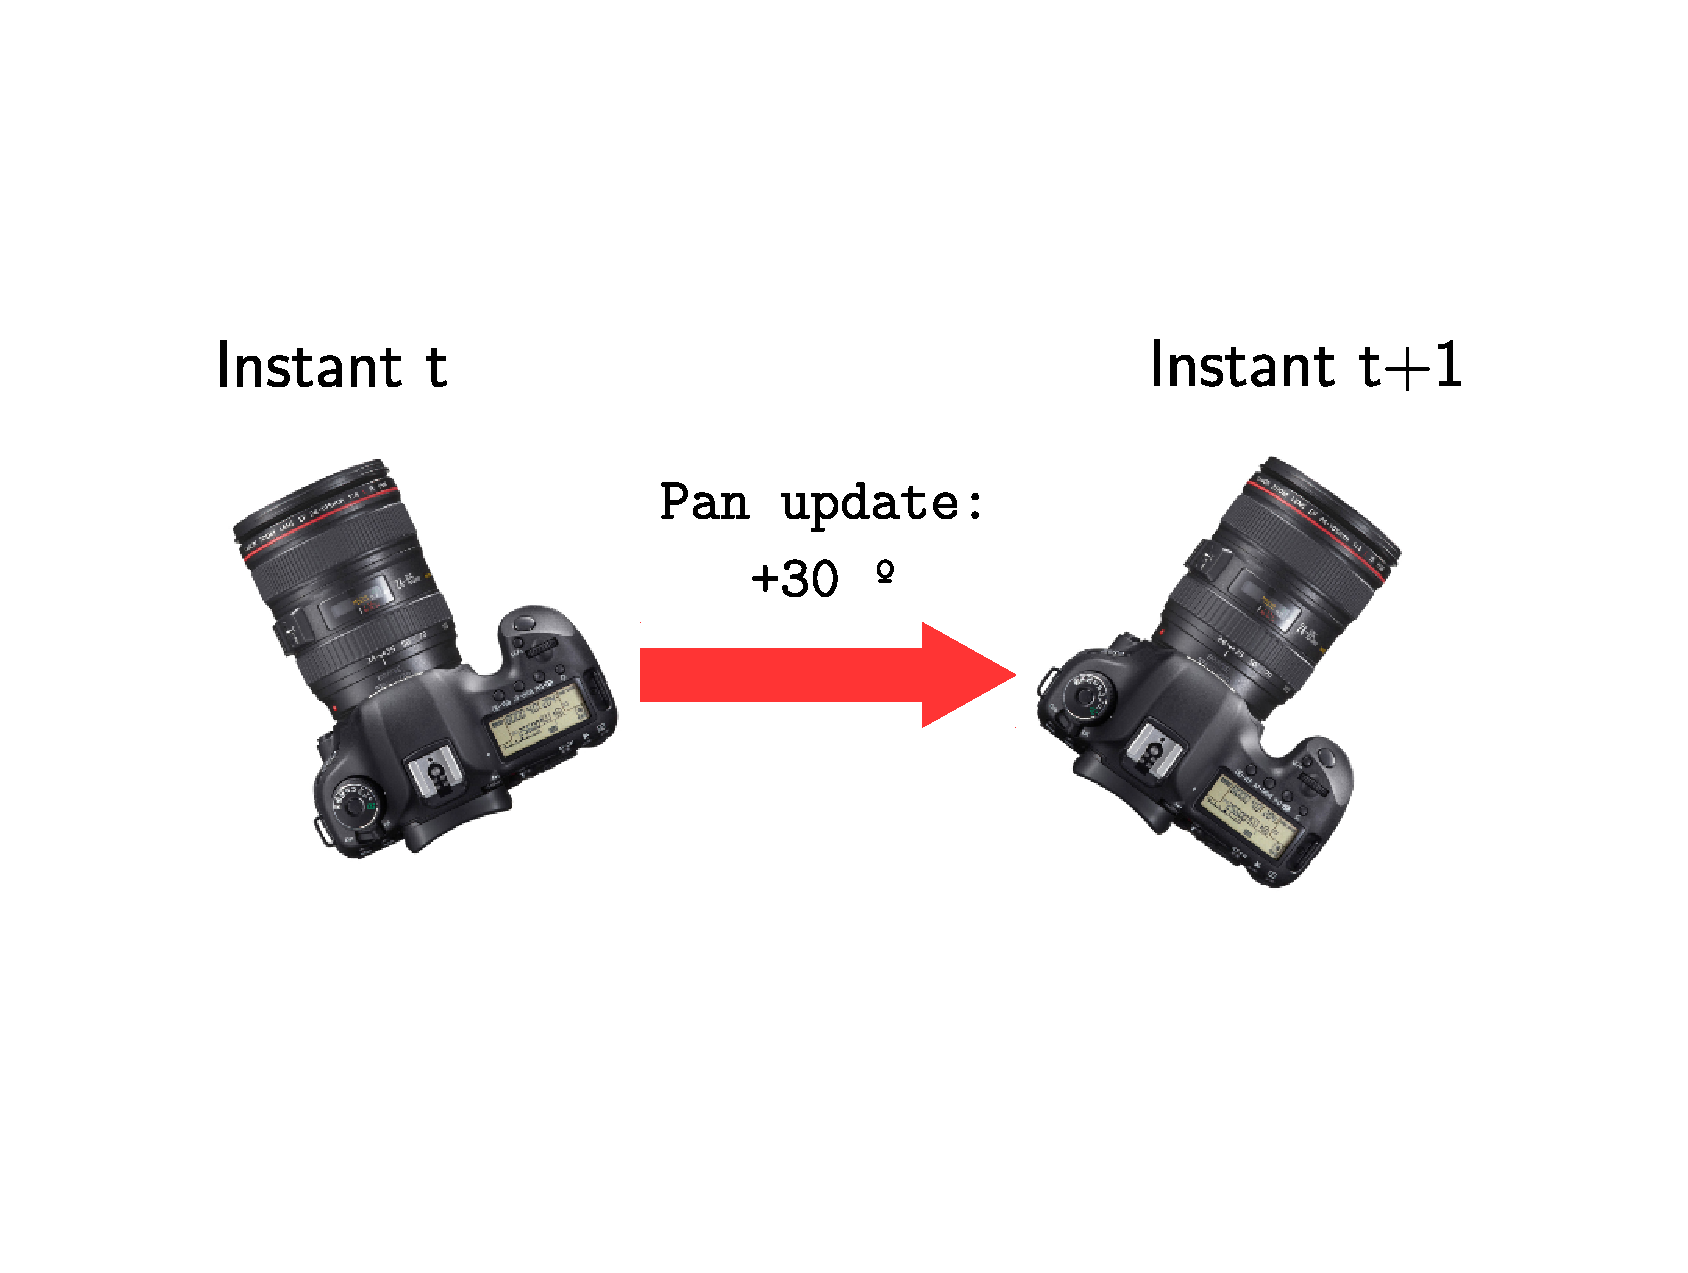
\includegraphics[width=2.7in]{images/ptz_wrong_movement}
				\caption{Wrong motion update (too long movements).}
				\label{fig:3_ptz_wrong}
			\end{subfigure}
			\qquad
			\begin{subfigure}[h]{0.4\linewidth}
				\centering
				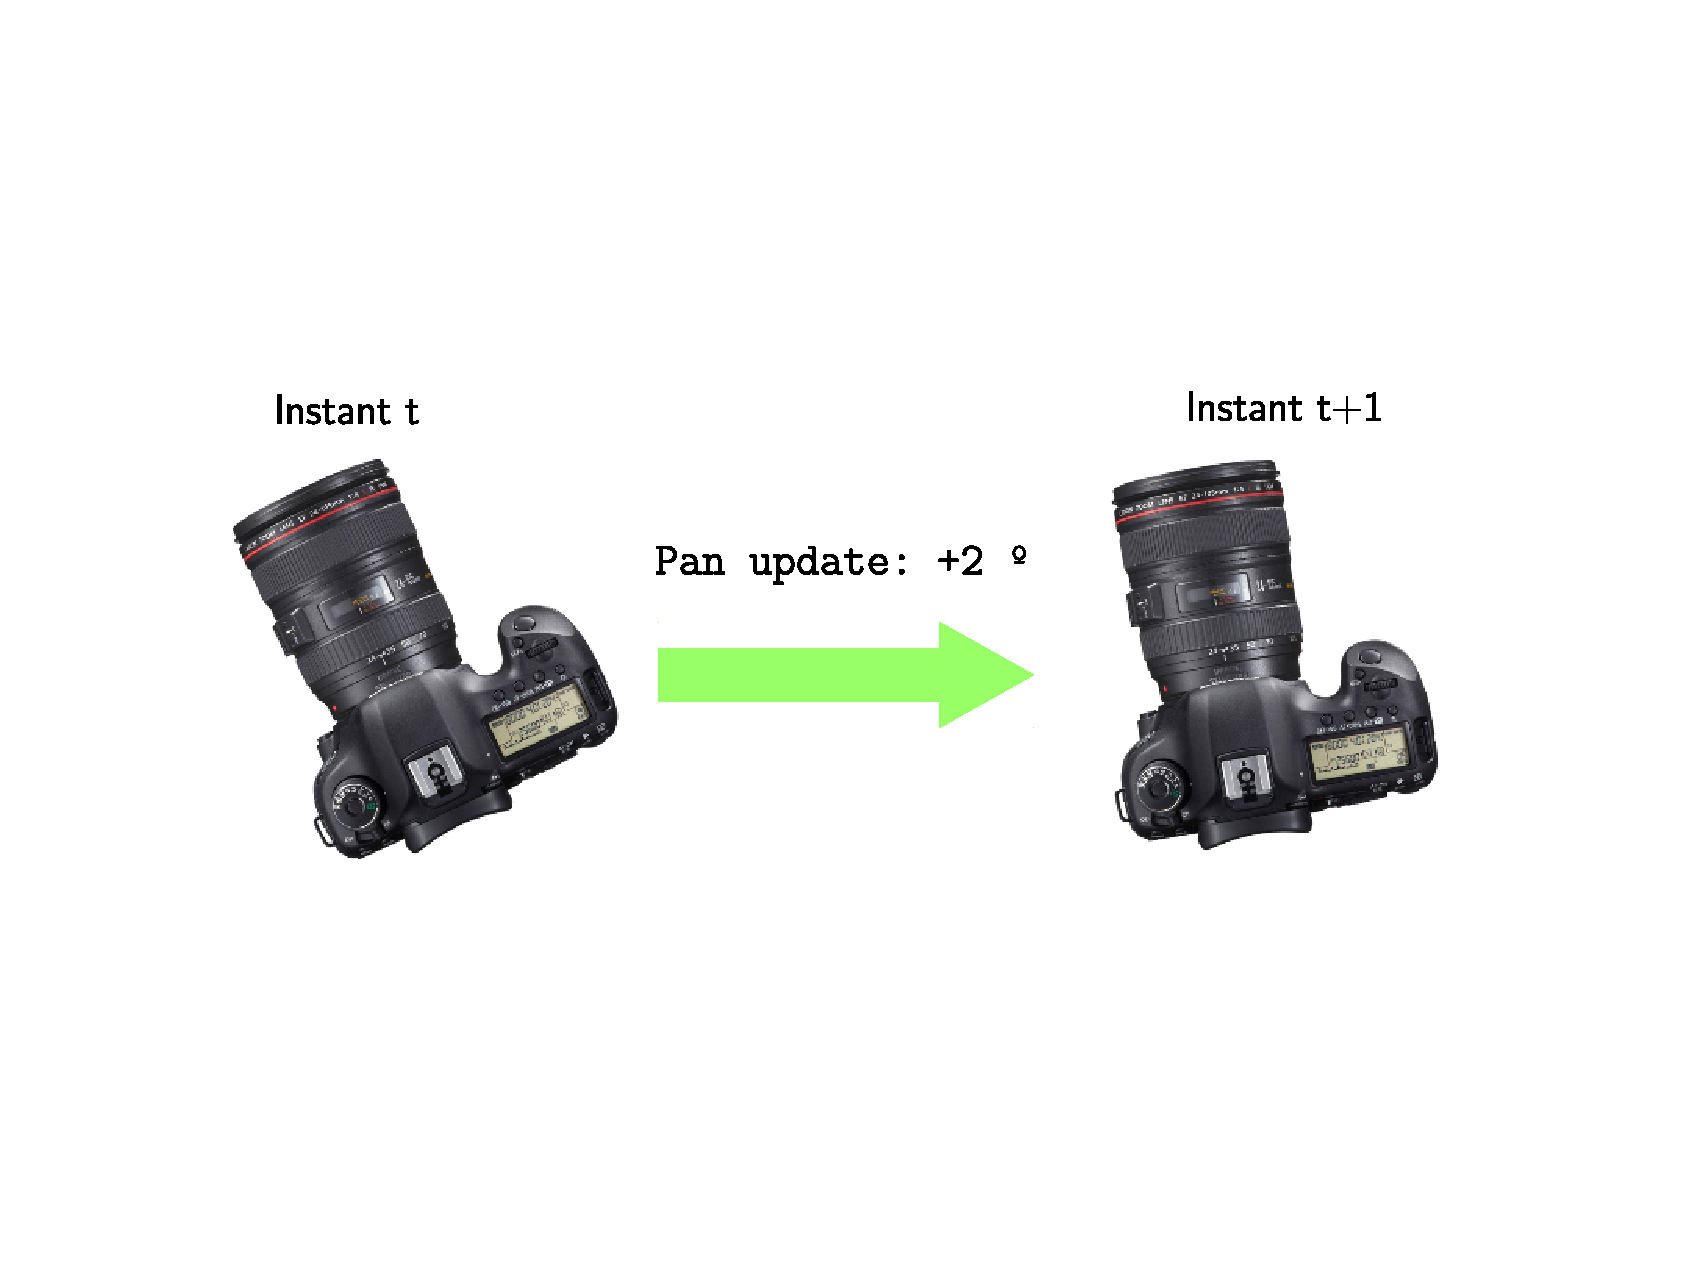
\includegraphics[width=2.7in]{images/ptz_correct_movement}
				\caption{Correct motion update (short differential movements).}
				\label{fig:3_ptz_right}
			\end{subfigure}
			\caption{Comparison between possible approaches for Pan/Tilt angle updates.}
			\label{fig:3_ptz_movements}
		\end{figure}
		

		This was the device we used for our first approximation to the sensing+actuating node (\autoref{sec:follow_ptz}), where the only response was moving the camera.\\

	\subsection{Asus Xtion Pro Live}
		It is a RGBD (RGB + Depth) sensor, designed by Asus for interactive PC applications development purposes. \\

		It has been our image source in the sensing+actuating node (\autoref{sec:follow_turtlebot}) we have developed. We used it in the second approximation (the response was the movement of the entire robot).

		\begin{figure}[h]
			\centering
			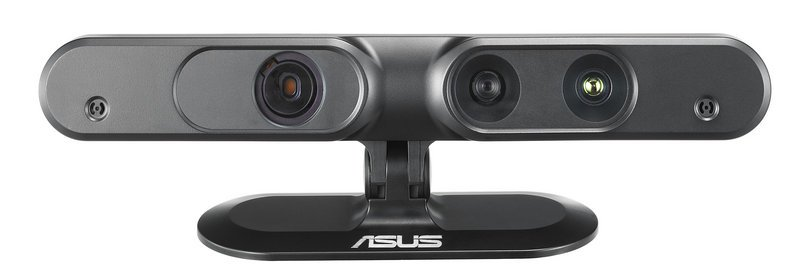
\includegraphics[width=0.4\linewidth]{images/xtion}
			\caption{Asus Xtion Pro Live. IR emitter (left), and RGB and IR lenses (right).}
			\label{fig:3_xtion}
		\end{figure}

		It counts on the left side with an IR (\emph{infrared}) light emitter, which radiates beams like a conventional light bulb (that's its function).\\

		On the right side, we can find two sensors:
		\begin{itemize}
			\item \emph{RGB sensor:} a conventional digital camera, with a resolution up to 1280x1024 px.
			
			\item \emph{Depth sensor:} it is capable of measure distance to objects, by receiving the reflections of the IR beams that we have mentioned above. It maps, for each pixel, the distance to that reflection (in mm), stored as a 16-bit long value.\\
			
			Thus, we can obtain a depth image, with a resolution of 640x480 px (@ 30 fps).
		\end{itemize}
		
		As it can be seen on \autoref{fig:3_xtion}, both sensor can't physically be in the same place, so there is a little discrepancy between both computed images:

		\begin{figure}[h]
			\centering
			\begin{subfigure}[h]{0.4\linewidth}
				\centering
				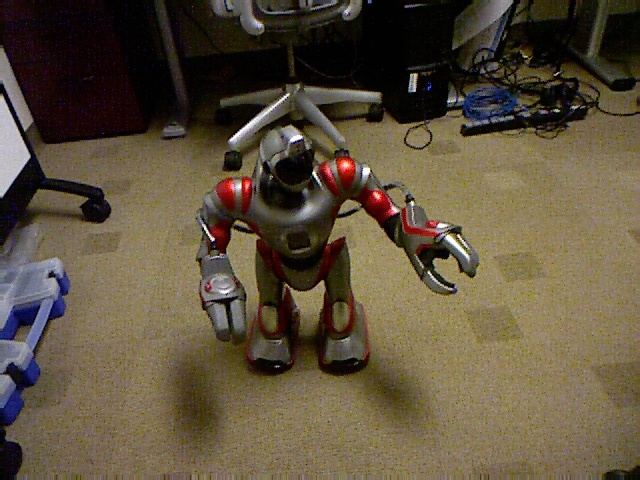
\includegraphics[width=3in]{images/rgb_before}
				\caption{RGB image.}
				\label{fig:3_rgb_bef_reg}
			\end{subfigure}
			\hfill
			\begin{subfigure}[h]{0.4\linewidth}
				\centering
				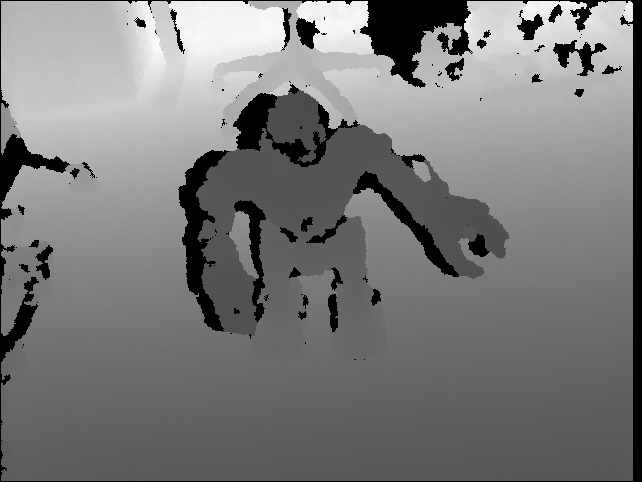
\includegraphics[width=3in]{images/depth_before}
				\caption{Depth image.}
				\label{fig:3_depth_bef_reg}
			\end{subfigure}
			
			\begin{subfigure}[h]{0.9\linewidth}
				\centering
				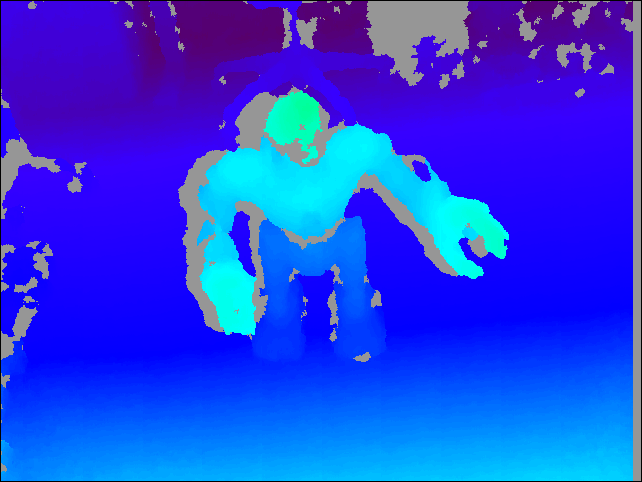
\includegraphics[width=3in]{images/disparity_before}
				\caption{Disparity (difference) between \ref{fig:3_rgb_bef_reg} and \ref{fig:3_depth_bef_reg}.}
				\label{fig:3_disparity_bef_reg}
			\end{subfigure}
			
			\caption{Both images sensed by the Xtion cameras, and the disparity between them \emph{before} the registration process.}
			\label{fig:3_bef_reg}
		\end{figure}
		
		With the goal of paliating this disparity, a process called \emph{registration} is executed for every new incoming depth image. It consists of a projection of the depth pixels into the RGB image, trying to align on an optimum way each pixel with its counterpart on the RGB image. We can observe that this can cancel to some degree the difference between both images (\autoref{fig:3_aft_reg}).
		
		
		\begin{figure}[h!]
			\centering
			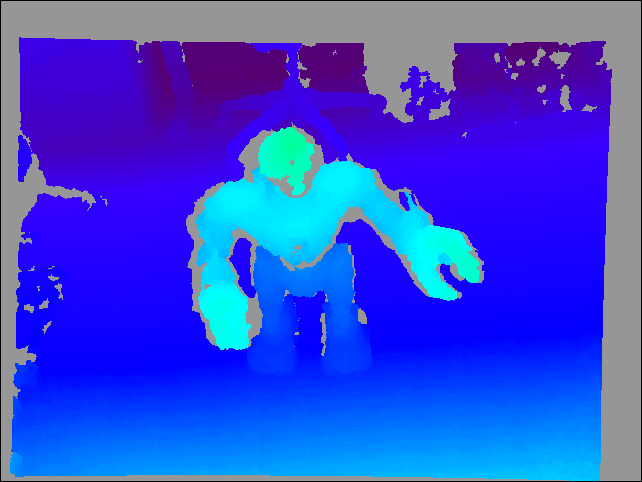
\includegraphics[width=3in]{images/disparity_after}
			\caption{Disparity between the images \emph{after} the registration process.}
			\label{fig:3_aft_reg}
		\end{figure}
		
		If we compare the new disparity (\autoref{fig:3_aft_reg}) with the previous disparity (\autoref{fig:3_disparity_bef_reg}), we can appreciate that now, the RGB and Depth images are aligned on an improved way, as if both sensors were on the same place, or much closer at least.\\
		
		So, from now on, we will call \emph{depth image} to the registered version of the depth map, as the unregistered image is not useful anymore.\\
		
		At last, we will make a mention to the open source drivers\footnote{\url{https://structure.io/openni}}, OpenNI (\emph{Open Natural Interaction}). They were originally developed by the Kinect developer company PrimeSense (which designed the Xtion device beside Asus).\\
		
		This interface allows to perform all the processes involved into handling this device (image grabbing, depth registration, etc.).
		
	\subsection{Turtlebot 2}
		The Turtlebot platform has been our main actuation platform on the developed actuation+response node (\autoref{chap:followperson}).\\
		
		\begin{figure}[h]
			\centering
			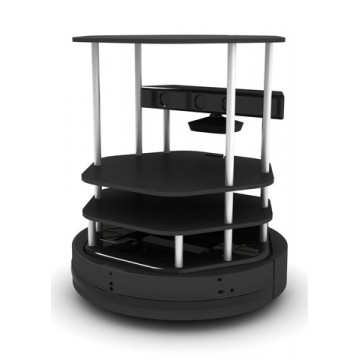
\includegraphics[width=3in]{images/turtlebot}
			\caption{Turtlebot development kit.}
			\label{fig:3_turtlebot}
		\end{figure}
		
		It is a research platform, composed by a structure jointed to a Kobuki robot (mobile base)\footnote{\url{http://kobuki.yujinrobot.com/about2/}}. Into this structure, there are also attached an Asus Xtion sensor (recently described), and a laser sensor, which has not been used on this project (nevertheless, it could be a continuation, as a navigation algorithm could be added to this project, on a similar way than in \cite{rocapal}).\\
	
		The user has the capability of connecting each of these devices via USB to the laptop, and place it at the top platform of the robot. From there, the computer can run the algorithm and command the movements. Every component can be handled with the respective ROS driver (which will be described later).
	

\section{Python}
	According to the official definition from \cite{python}, Python is \textit{an interpreted, object-oriented, high-level programming language with dynamic semantics}. It was created in 1991 by Guido van Rossum (who consecrated its name to the TV series \textit{Monty Python}). However, due to the increasing growth of \emph{Machine Learning} that happened the last two decades, it has become the most popular language for this purpose, due to its focus on \emph{easiness}, its duck typing\footnote{This refers to Python guessing about your variables, coming from the phrase \textit{''if it looks like a duck and sounds like a duck, chances are it's a duck."}} and its strong Object Orientation: everything can be treated as an object on this language. This is a very interesting feature, as it facilitates features as sharing memory, abstract processes, and much more.
	
	And, of course, it is \textit{Open Source}, so it is always under community improvements, and there are a vast number of incredibly useful third party libraries, which are impossibly easier to deploy onto your code.\\
	
	This makes this language a really potential candidate for the applications to develop (and that's precisely the reason that explains its huge growth on the software market).\\
	
	For our target, we will use Python on its version $2.7$. Although it is a relatively old version of the language, it is necessary to mantain the compatibility with ROS (\autoref{sec:3_ros}) bindings, which have not still taken the leap to the newest major version ($3.x$) on Python.\\
	
	Nevertheless, we want to mention the fact that Python is an \emph{interpreted} language, which means that its sentences are projected on another program (the Python interpreter, which executes them), and not directly by the processing hardware (CPU/GPU). This can be a con, as it makes the code execution much slower, in comparison with standard \emph{compiled} languages, which are run directly as processes, and taken by the computer hardware for its execution (as C, C++, Picky, etc.).

\section{ROS}
	\label{sec:3_ros}
	As it is said on \cite{ros-intro}, \emph{ROS} (Robot Operating System) is \textit{an open-source, meta-operating system for your robot}, maintained by the \emph{OSRF} (Open Source Robotics Foundation). It is a framework that provides a distributed, easily-scalable environment of \emph{nodes}. These nodes are programs which are independently running on the computer (or distributed over a P2P network), so they can perform individual tasks. However, they can communicate between themselves on a synchronous way (over \emph{services}, implementing a client-server role system between nodes), or on an asynchronous way, via \textbf{topics}, which will be the main benefit we will take advantage of. These topics, which rely on a standard TCP/UDP communication between sockets via the \texttt{loopback} interface, are intended for an unidirectional, streaming communication, where a node can take a role: \emph{publisher} (if it is writing data inside the topic), or \emph{subscriber} (if it is reading the data that publishers are broadcasting into the topic). The data flow through the topic, however, is not unrestricted. It must follow a ROS specific syntax, the \emph{Message} type, which is strictly defined for the communication purpose (geometry, sensoring, etc.).\\
	
	For our project we will be using the 2016 \textit{LTS} (Long Term Support) version, called \textit{Kinetic Kame}\footnote{\url{http://wiki.ros.org/kinetic}}. This is the version bundled on the installation of JdeRobot\footnote{\url{https://jderobot.org/Installation}}.\\
	
	ROS provides libraries and bindings for C++, Lisp, and \textit{Python} (\texttt{rospy}). They allow, among plenty of other stuff, to really easily set up a topic between two or more programs, which will be seen as ROS nodes.\\
	\begin{figure}[h]
		\begin{lstlisting}
...
import rospy
from std_msgs.msg import String
...
rospy.init_node('listener')              # Starting the node entity.
rospy.Subscriber('chatter', String)      # Instantiation of the topic subscriber.
rospy.spin()                             # 'Infinite loop' listening to the topic.
...
		\end{lstlisting}
		\caption{Simple stablishment of a listener node through \texttt{rospy} (code from \cite{listener-rospy}).}
		\label{fig:3_rospy_listener}
	\end{figure}
	
	However, this topic communication will be abstracted on our project by the \texttt{comm} library, as it will be seen on \autoref{sec:3_comm}.\\
	
	ROS also provides a Debian package, called \texttt{rosbash}, which allows to, in a very handy way, manage nodes and packages from a standard \texttt{bash} shell. The most remarkable feature for us is the command \texttt{roslaunch}, that launches a ROS node with a certain specific settings, configurable via a \texttt{.launch} file (which follows a XML formatting). An example for the file structure can be found on \autoref{fig:3_launch_file}.\\
	
	\subsection{\texttt{usb\_cam}}
	\label{sec:3_usb_cam}
		ROS node that creates a topic and publishes into it the digital video data incoming from a USB camera, into the topic \texttt{/usb\_cam/image\_raw}.\\
		
		This node will be used on the first approach to the sensing+actuating node (\autoref{sec:follow_ptz}), with the purpose of retrieving images from the Sony EVI D100P camera (\autoref{fig:3_evi}). In consequence, a custom configuration file\footnote{\url{https://github.com/RoboticsURJC-students/2017-tfg-nacho\_condes/blob/master/resources/usb\_cam-test.launch}} is required. We can have a glance on that configuration file (\autoref{fig:3_launch_file}).\\
		
		\begin{figure}[h]
			\centering
			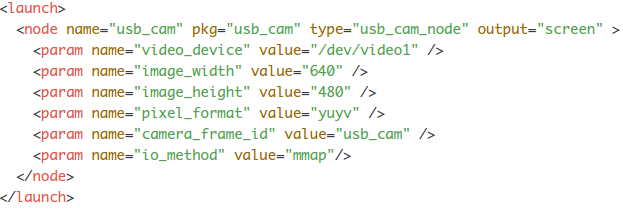
\includegraphics[width=5in]{images/usb_cam_test}
			\caption{Example of \texttt{usb\_cam-test.launch} configuration file for a ROS node.}
			\label{fig:3_launch_file}
		\end{figure}
		\begin{center}
			Usage: \texttt{roslaunch usb\_cam-test.launch}
		\end{center}

	\subsection{\texttt{openni2\_launch}}
		This ROS binding \cite{openni2-doc} provides the launch files for the \texttt{rgbd\_launch} node. This node publishes on several topics the RGB+D images provided by the Asus Xtion (\autoref{fig:3_xtion}), performing at the same time the registration process.\\
		
		This node will be used on the second iteration of the sensing+actuating node (\autoref{sec:follow_turtlebot}). It will connect the Xtion sensor to the component, providing the real-time imaging through the topic.\\

		\begin{center}
			Usage: \texttt{roslaunch openni2\_launch openni2.launch}
		\end{center}
		

	\subsection{\texttt{kobuki\_node}}
		This ROS package contains a bunch of launch files. Among them there is the one we will use: \texttt{minimal.launch}, which starts the \emph{nodelet}\footnote{A ROS nodelet performs multiple simultaneous processes, and consequently opens several topics.} that gives us the total control of the Kobuki robot connected to the computer\footnote{We refer to the robot as \emph{Kobuki} now because the mobile base of the Turtlebot (\autoref{fig:3_turtlebot}) is the only ROS device which we will control in our application.}.\\
		
		This node will be used on the second iteration of the sensing+actuating node (\autoref{sec:follow_turtlebot}). It will connect the Turtlebot motors to the component, providing the topic to command movements to them.
		
		\begin{center}
			Usage: \texttt{roslaunch kobuki\_node minimal.launch}
		\end{center}

	
\section{JdeRobot}
	As described in \autoref{sec:dl_jderobot}, JdeRobot\footnote{\url{https://jderobot.org}} is a distributed development platform/middleware, born in \cite{jmplaza-phd}. It stands out mainly for two key aspects:
	\begin{itemize}
		\item \textit{Hardware abstraction:} it behaves as an intermediate layer between control software (written by the programmer) and hardware, which can be a real device (a robot, drone, camera, laser scanner, etc.), or a simulation (on the open source world simulator Gazebo\footnote{\url{http://gazebosim.org/}}). This way, the bidirectional flow (information from sensors, and commands from the computer) is sent the same way, \textit{no matter the kind of the robotic device}.
		
		As well, this abstraction layer allows various computers to interact simultaneously with the hardware, as the communications are also abstracted to ROS topics or ICE endpoints (it will be properly explained at \autoref{sec:3_comm}), where a program has to just listen/talk to be in on. This provides a very valuable \textit{software and hardware scalability to the platform, and to the developed programs}.\\
		
		Let's have a look on a possible example on the \autoref{fig:3_jderobot_hal}. This could represent an scenario where somebody wants to virtually test a navigation algorithm. Thus, in the \emph{Computer 1}, a reactive controller is running, sensing the environment through a real laser scanner and a RGB camera (as in the work developed at \cite{rocapal}). This controller receives data from the sensors, computes a proper navigation response, and sends it to a virtual robot, simulated on Gazebo.
		
		Additionally, another machine (\emph{Computer 2}) is running a viewer, which allows it to draw the images seen by the camera, and the laser readings from the scanner. So, this component only receives the data from the sensors, and does not send any kind of data to the devices.
		
		We can see that both components can perfectly run together and on different machines, even when they are written over completely different languages (Python and C++, respectively). In addition, we can perfectly handle virtual and real devices simultaneously, even if they talk through different interfaces (ROS or ICE), due to the perfect support of this division by the \texttt{comm} (\autoref{sec:3_comm}) library.\\
		
		
		\begin{figure}[h!]
			\centering
			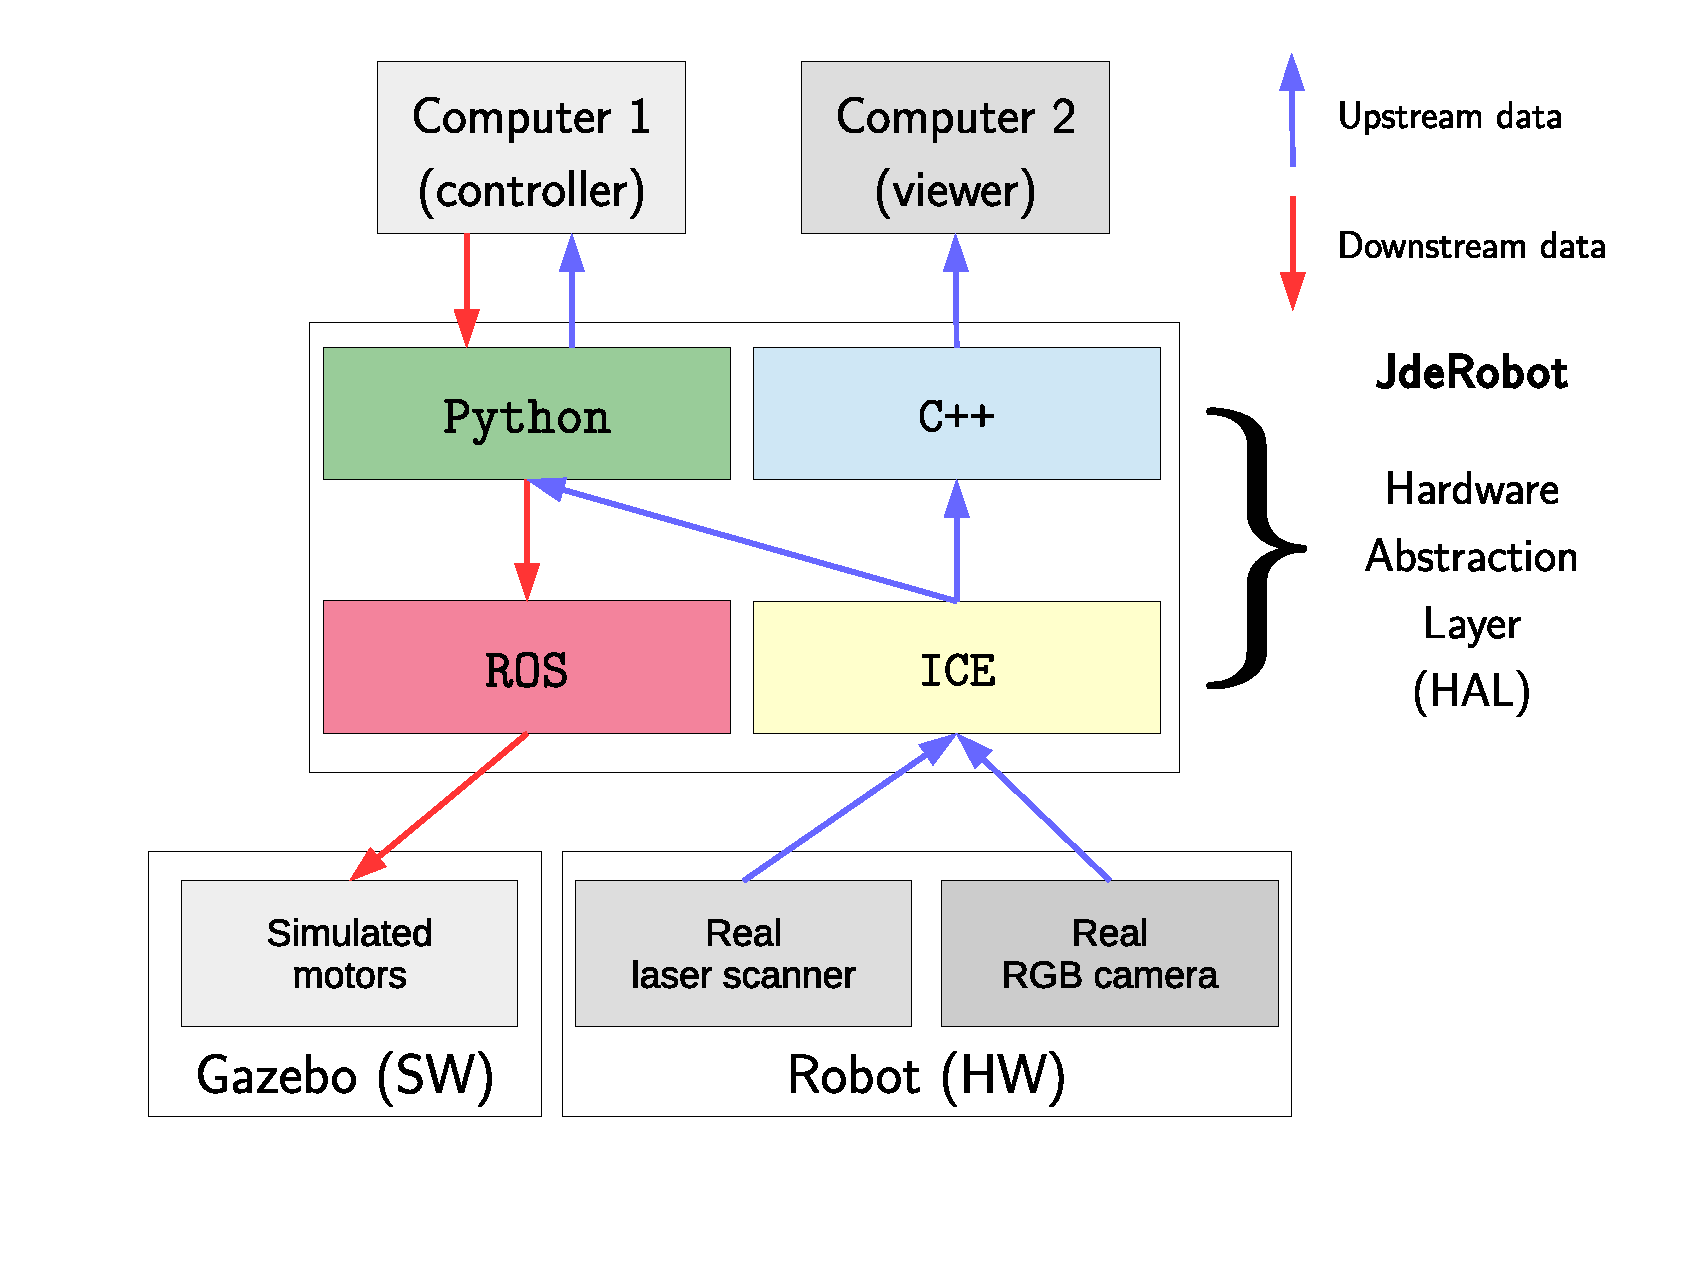
\includegraphics[width=4in]{images/jderobot_hal}
			\caption{JdeRobot abstraction layer, and a possible use distributed, multi-middleware scenario.}
			\label{fig:3_jderobot_hal}
		\end{figure}
		
		 \textit{So, in this easiness and flexibility resides the main advantage of using JdeRobot}.
		
		\item \textit{Wide device support:} JdeRobot provides full compatibility with ROS Kinetic Kame, so it can perfectly integrate with ROS Nodes (in our concern, we can communicate with the Turtlebot and the Xtion devices via several topics that the ROS intermediate nodes open).
		
		\item \textit{Behavioral based on threaded parallel schemes:} as it is introduced at  \cite{jmplaza-phd}, inside a component, we will find one or more \emph{schemes}, objectified on threads. These threads run concurrently with an specific timing (so it does not overload the CPU in vain if a few iterations per second are enough for a vivacious and correct response).\\
		
		These schemes perform different tasks each, as seen on \autoref{fig:2_tasks} on a non-blocking way, and share memory. This has been followed on a comfortable way on our implementation: the threads are independent, but the tasks they control are performed by Python objects, which are interconnected between them:
		
		As an example, we can see how this has been performed inside our Python code:
		
		\begin{figure}[h]
			\centering
			\begin{lstlisting}
...
cam = Camera(ros_topic)           # Creation of the camera.
net = Network(graph_model)        # Creation of the CNN.

net.setCamera(cam)                # Connection of the camera and the CNN,
                                  # which now can share memory.

t_cam = ThreadCamera(cam)         # Instantiation and start of the thread which
t_cam.start()                     # implements the Camera schema.

t_net = ThreadNetwork(net)        # Instantiation and start of the thread which
t_net.start()                     # implements the Network schema.
...
			\end{lstlisting}
			\caption{Handling schemes on Python with objects and threads.}
			\label{fig:3_schemes_python}
		\end{figure}
	\end{itemize}
	
	\vspace{0.4in}
	
	To sum up, we have described the goodness of the JdeRobot framework for our purposes, and seen how we can implement the \textit{useful schemes paradigm} on an easy way into Python, our development language.\\
	
	Now, in the next subsections, we will examine which of the JdeRobot components, apart of the structure, have been of greatest interest for us.
	
	\subsection{Digit Classifier}
	\label{sec:3_digitclassifier_jderobot}
		This JdeRobot component\footnote{\url{https://github.com/JdeRobot/dl-digitclassifier}} was originally designed by David Pascual \cite{dpascualhe} and Nuria Oyaga \cite{noyaga}, and it was used on this project to land on the concept of neural networks.\\
		
		Its design aims to \textit{classify handwritten numbers} with the use of a Convolutional Neural Network (\autoref{sec:1_cnn}), that classifies the incoming images from a video source.\\
		
		\begin{figure}[h]
			\centering
			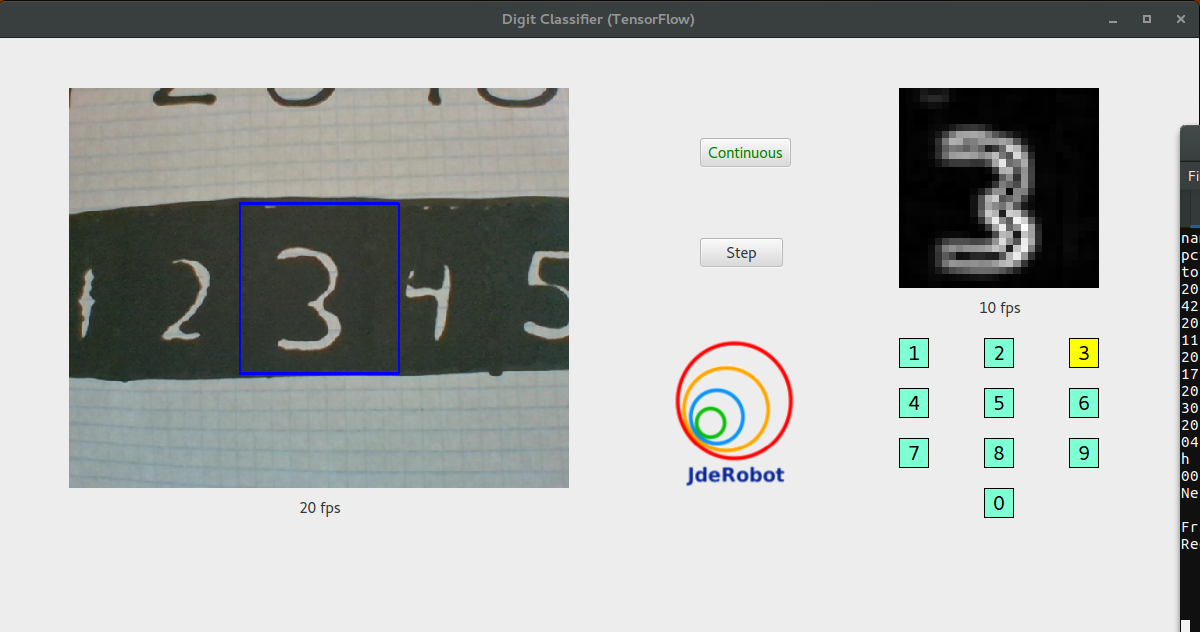
\includegraphics[width=4in]{images/digitclassifier}
			\caption{\texttt{DigitClassifier} on action.}
			\label{fig:3_digitclassifier}
		\end{figure}
		
		The previous implementations were written in Keras and Caffe (Python libraries to implement Neural Networks), so we made the same on TensorFlow (\autoref{sec:3_tensorflow}), to accomplish an initial domain of this Machine Learning framework.\\
		
		The implementation of this convolutional neural network consists on a concatenation of layers, following the scheme shown on \autoref{fig:3_digitclassifier_neural_structure}, which perform specific operations.
		
		\begin{figure}[h]
			\centering
			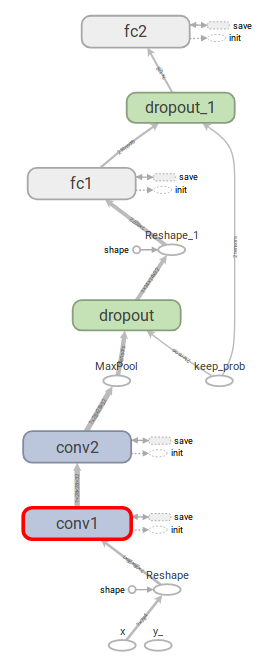
\includegraphics[width=2in]{images/digitclassifier_network_graph}
			\caption{Digit classifying neural structure.}
			\label{fig:3_digitclassifier_neural_structure}
		\end{figure}



		\begin{enumerate}
			\item \texttt{conv1}: first convolutional layer. As described in \autoref{sec:1_cnn}, it performs a 2D convolution between a $5px \times 5px$ square mask\/kernel (\texttt{W\_conv1}), and then adds a bias/intercept term (\texttt{b\_conv1}).\\
			\item \texttt{conv2}: second convolutional layer. It performs the same operation taking the output from the previous layer as an input, using a different weights mask and bias terms.\\
			
			Until now, what we have done is extracting patterns on each digit type (e.g. discovering typical circles on $0$ and $8$, which are always present on the same zone of the image).\\
			\item \texttt{pooling}: as the activation maps can be growing in size as we perform feed forward propagation, a \emph{pooling} operation is performed. It consists on sampling the input. Concretely, we retain the \textit{maximum} value for each 2 pixels, which is known as \textit{$2x2$ \texttt{max pooling}}
			
			\item \texttt{dropout}: this layer does not strictly perform any mathematical operations. It lets pass the TENSORS through it, but randomly switching off some neurons. This is parameterized by a user input, using a variable called \texttt{keep\_prob}. In our case, we set it to $0.5 (50\%)$ during the training process, to avoid overfitting by forcing the network to modify the neural paths randomly, as not every neuron is available on every moment. This is kind of similar to augmenting the dataset during the training process. The rest of the time (when the network is used to make inferences), this parameter is set to $1.0$, which means that no neurons are switched off at all.\\
			\item \texttt{fc1}: first fully connected layer. These layers, also known as \emph{dense} layers, are distinguised because every neuron is connected to every activation from the previous layer. So, this kind of layers are used for \text{pattern association with labels}, due to the relationship they can infer between every input.\\
			\item \texttt{fc2}: the output layer. It connects all the outputs of the previous dense layer and groups the output in a 10-dimensional vector, which contains the probability of the digit to belong to each one of the possible classes.
		\end{enumerate}


		
		Once all this was achieved, we upgraded the code (from single ICE support to ROS+ICE via the \texttt{comm} library), and unified it (Keras + TensorFlow frameworks in a single component, under choice using the YML configuration file) on the official JdeRobot repository. From there it can be used right out of the box with the included model for both frameworks. In addition, you can train your own models using the provided datasets, or yours if you build another.
	
	
	\subsection{\texttt{evicam\_driver}}
	\label{sec:3_evicam_driver}
	This driver, bundled into JdeRobot\footnote{\url{https://github.com/JdeRobot/JdeRobot/tree/master/src/drivers/evicam\_driver}}, allows the user to send movements commands to a Sony EVI D100P camera \autoref{fig:3_evi}) and retrieve information from it, creating an ICE endpoint that is ready to interact with the camera \emph{PT} (Pan, Tilt) motors.\\
	
	As this is a low-level driver, written in C++, it requires to be used on a specific way, which has been documented\footnote{\url{https://jderobot.org/Handbook\#PanTilt_Teleop}} to be easily applied in the future.\\
	
	This driver defines an interaction API with the camera, which allows us to get the values from the motors encoders:
	\begin{lstlisting}
import config
import comm
...

cfg = config.load('yml_configuration_file')
jdrc = comm.init(cfg, 'NodeName')


# Instantiation for the motors:
PTMotors = jdrc.getPTMotorsClient('NodeName.PTMotorsEndpoint')

print(PTMotors.getLimits()) # Shows the max/min values for pan, tilt 
                            # and each speed.

print(PTMotors.motors.data) # Shows the current values for pan, tilt
                            # and each speed.

# Let's move the camera! As easy as:
PTMotors.setPTMotorsData(new_pan, new_tilt, max_pan_speed, max_tilt_speed)
	\end{lstlisting}
	
	\subsection{\texttt{comm}}
		\label{sec:3_comm}
		\texttt{comm} is the basic library to perform communications between different components. It is what supports all the data flows in a typical scenario (\autoref{fig:3_jderobot_hal}).\\
		
		\texttt{comm} consists on a collection of bindings to easily create a link between two components, or between a device and a component. On the lowest level, we can use it relying on ROS (through topics as it was explained before on \autoref{sec:3_ros}), or through an ICE proxy. ICE\footnote{\url{https://zeroc.com/products/ice}} is an object-oriented middleware that, in our purpose, allows to abstract a data flow to a TCP/IP endpoint (an address/hostname, and a port), which can even support a communication between two or more programs inside the same machine.\\
		
		To create a communicator with \texttt{comm}, it needs the specification for that link (underlying middleware, topic/endpoint, etc.), so it uses the JdeRobot standard: YML\footnote{Legible data serialization format.} configuration files, which can be like in \autoref{fig:3_yml_format}.
		\begin{figure}[h]
			\centering
			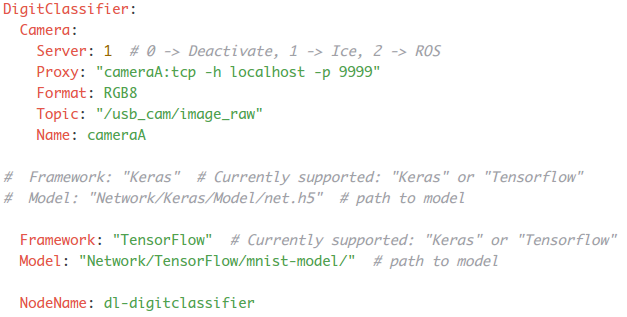
\includegraphics[width=4in]{images/yml_format}
			\caption{YML format on the \texttt{digitclassifier.yml} file.}
			\label{fig:3_yml_format}
		\end{figure}
		
\section{OpenCV}
\section{TensorFlow}
\label{sec:3_tensorflow}
\section{Keras}
\section{PyQt (v.5)}
\section{Threading}

	
	\chapter{\texttt{DigitClassifier} node}
	\label{chap:4_digitclassifier}
	\section{Description}
	\section{Functional architecture}
	\section{Neural Network processing}
		This JdeRobot component\footnote{\url{https://github.com/JdeRobot/dl-digitclassifier}} was originally designed by David Pascual \cite{dpascualhe} and Nuria Oyaga \cite{noyaga}, and it was used on this project to land on the concept of neural networks.\\
		
		Its design aims to \textit{classify handwritten numbers} with the use of a Convolutional Neural Network (\autoref{sec:1_cnn}), that classifies the incoming images from a video source.\\
		
		\begin{figure}[h]
			\centering
			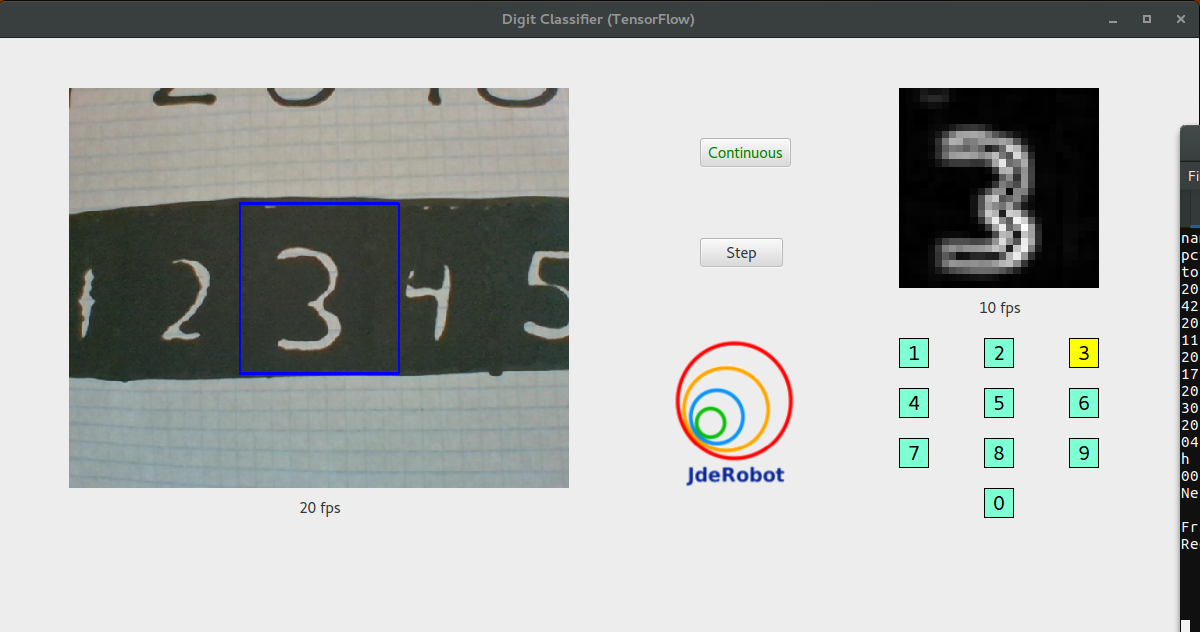
\includegraphics[width=4in]{images/digitclassifier}
			\caption{\texttt{DigitClassifier} on action.}
			\label{fig:4_digitclassifier}
		\end{figure}
			
			The previous implementations were written in Keras and Caffe (Python libraries to implement Neural Networks), so we made the same on TensorFlow (\autoref{sec:3_tensorflow}), to accomplish an initial domain of this Machine Learning framework.\\
			
			The implementation of this convolutional neural network consists on a concatenation of layers, following the scheme shown on \autoref{fig:3_digitclassifier_neural_structure}, which perform specific operations.
			
			\begin{figure}[h]
				\centering
				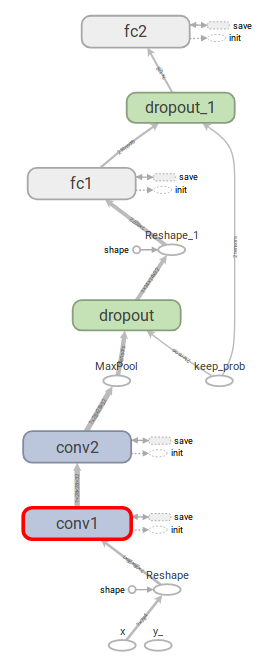
\includegraphics[width=2in]{images/digitclassifier_network_graph}
				\caption{Digit classifying neural structure.}
				\label{fig:3_digitclassifier_neural_structure}
				\end{figure}
				
				
				
				\begin{enumerate}
					\item \texttt{conv1}: first convolutional layer. As described in \autoref{sec:1_cnn}, it performs a 2D convolution between a $5px \times 5px$ square mask\/kernel (\texttt{W\_conv1}), and then adds a bias/intercept term (\texttt{b\_conv1}).\\
					\item \texttt{conv2}: second convolutional layer. It performs the same operation taking the output from the previous layer as an input, using a different weights mask and bias terms.\\
					
					Until now, what we have done is extracting patterns on each digit type (e.g. discovering typical circles on $0$ and $8$, which are always present on the same zone of the image).\\
					\item \texttt{pooling}: as the activation maps can be growing in size as we perform feed forward propagation, a \emph{pooling} operation is performed. It consists on sampling the input. Concretely, we retain the \textit{maximum} value for each 2 pixels, which is known as \textit{$2x2$ \texttt{max pooling}}
					
					\item \texttt{dropout}: this layer does not strictly perform any mathematical operations. It lets pass the TENSORS through it, but randomly switching off some neurons. This is parameterized by a user input, using a variable called \texttt{keep\_prob}. In our case, we set it to $0.5 (50\%)$ during the training process, to avoid overfitting by forcing the network to modify the neural paths randomly, as not every neuron is available on every moment. This is kind of similar to augmenting the dataset during the training process. The rest of the time (when the network is used to make inferences), this parameter is set to $1.0$, which means that no neurons are switched off at all.\\
					\item \texttt{fc1}: first fully connected layer. These layers, also known as \emph{dense} layers, are distinguised because every neuron is connected to every activation from the previous layer. So, this kind of layers are used for \textit{pattern association with labels}, due to the relationship they can infer between every input.\\
					\item \texttt{fc2}: the output layer. It connects all the outputs of the previous dense layer and groups the output in a 10-dimensional vector, which contains the probability of the digit to belong to each one of the possible classes.
					\end{enumerate}
					
					
					
					Once all this was achieved, we upgraded the code (from single ICE support to ROS+ICE via the \texttt{comm} library), and unified it (Keras + TensorFlow frameworks in a single component, under choice using the YML configuration file) on the official JdeRobot repository. From there it can be used right out of the box with the included model for both frameworks. In addition, you can train your own models using the provided datasets, or yours if you build another.
					


\chapter{\texttt{ObjectDetector} node}
\section{Description}
\section{Functional architecture}
\section{Neural Network processing}


\chapter{\texttt{FollowPerson} node}
\label{chap:followperson}
\section{Description}
\section{Functional architecture}
\section{Neural Network processing}
\section{Face detection and identification}
\section{Tracking algorithm}
\section{Physical response (\emph{PID} controller)}
\section{Experiments}
\subsection{Alternative approach: PTZ Camera}
\label{sec:follow_ptz}


\chapter{Conclusions}
	\section{Conclusions}
	\section{Future research lines}
	
	
	%%%%%%%%% BIBLIOGRAPHY %%%%%%%%%
	\bibliography{bibliography}
	\bibliographystyle{unsrt}
\end{document}